\documentclass[a4paper,10pt]{ctexart}
%引用设置使用Bibtex
\usepackage{gbt7714}
\bibliographystyle{gbt7714-numerical}
%页面设置
\usepackage{geometry}
%字体设置
\usepackage{fontspec}
%\setmainfont{Times New Roman}
%定理环境
\usepackage{amsmath}
\numberwithin{equation}{section}
\usepackage{amsthm}
\newtheorem*{definition}{Definition}
\newtheorem{theorem}{Theorem}
\newtheorem{lemma}{Lemma}
\newtheorem*{corollary}{Corollary}
\newtheorem*{proposition}{Proposition}
\newtheorem*{example}{Example}
%数学环境字体
\usepackage{bm}
\usepackage[all]{xy}
%加载 TikZ 用于绘制交换图
\usepackage{tikz-cd}
\usepackage{tikz}
\usepackage{pgfplots}
\newcommand{\tikzdef}{\pgfmathsetmacro} % 在tikzpicture内的foreach循环中定义实数临时变量
%颜色
\usepackage{color,xcolor}

\definecolor{miku}{RGB}{57,197,187}
\definecolor{sakura}{RGB}{255,192,203}
\definecolor{rose}{RGB}{255,228,225}
\definecolor{brown}{RGB}{210,105,30}
\definecolor{lbrown}{RGB}{239,235,224}
\definecolor{bule}{RGB}{0,47,167}
\definecolor{lyellow}{RGB}{250,250,210}
\definecolor{lpurple}{RGB}{255,240,245}
\definecolor{lbule}{RGB}{135,206,250}
\definecolor{gbule}{RGB}{64,224,208}
\definecolor{green}{RGB}{138,200,207}
\definecolor{lgreen}{RGB}{225,255,255}
\definecolor{lorange}{RGB}{248,172,140}
\definecolor{salmon}{RGB}{250,128,114}
\definecolor{burgundy}{rgb}{0.5, 0.0, 0.13}
%链接设置
\usepackage[colorlinks=true,pdfstartview=FitH,linkcolor=blue,anchorcolor=violet, citecolor=magenta]{hyperref} 
%封面
\usepackage{pdfpages}
\usepackage{mathrsfs}
\usepackage{amssymb}
\usepackage{graphicx}
\usepackage{lipsum}
%彩色框
\usepackage{framed}
\usepackage{tcolorbox}
\tcbuselibrary{breakable}
\tcbuselibrary{theorems}
\tcbuselibrary{skins}
\usepackage{colortbl}
\usepackage{float}
\usepackage[export]{adjustbox}
\newtcolorbox[auto counter,number within=section]{notebox}[2][]{%
colback=miku!2!white,
colframe=miku,
coltitle=white,
fonttitle=\bfseries,
rightrule=2pt,
leftrule=2pt,
bottomrule=2pt,
colbacktitle=miku,
theorem style=standard,
breakable,
arc=2pt,
drop fuzzy shadow=black!20!white,
title=Note~\thetcbcounter: #2,#1}
\newtcolorbox[auto counter,number within=section]{markbox}[2][]{%
colback=miku!2!white,
colframe=miku,
coltitle=white,
fonttitle=\bfseries,
rightrule=0pt,
leftrule=0pt,
bottomrule=2pt,
colbacktitle=miku,
theorem style=standard,
breakable,
arc=0pt,
drop fuzzy shadow=black!20!white,
title=Remark~\thetcbcounter: #2,#1}
\newtcolorbox[no counter]{theorems}[2][]{%
width=12cm,
center,
sidebyside,
sidebyside adapt=left,
sidebyside gap=6mm,
sidebyside align=center seam,
colback=burgundy!2!white,
colframe=burgundy,
coltitle=white,
fonttitle=\bfseries,
rightrule=1pt,
leftrule=1pt,
bottomrule=2pt,
colbacktitle=burgundy,
theorem style=standard,
enhanced,
drop fuzzy shadow southeast=black!30!white,
breakable,
arc=0pt,
title=Theorem. #2,#1}
\newtcolorbox[no counter]{definitions}[2][]{%
width=12cm,
center,
colback=lyellow!2!white,
colframe=yellow!3!lyellow,
coltitle=bule,
fonttitle=\bfseries,
rightrule=0pt,
leftrule=1pt,
bottomrule=2pt,
colbacktitle=lyellow,
theorem style=standard,
breakable,
arc=5pt,
enhanced,
drop fuzzy shadow southeast=black!20!white,
title=Definition. #2,#1}
\newtcolorbox[auto counter,number within=section]{corollarys}[2][]{%
colback=lyellow!2!white,
colframe=lyellow,
coltitle=bule,
fonttitle=\bfseries,
rightrule=0pt,
leftrule=1pt,
bottomrule=2pt,
colbacktitle=lyellow,
theorem style=standard,
breakable,
arc=0pt,
enhanced,
drop fuzzy shadow southeast=black!20!white,
title=Corollary~\thetcbcounter: #2,#1}
\newtcolorbox[auto counter,number within=section]{lemmas}[2][]{%
width=12cm,
center,
colback=lyellow!2!white,
colframe=lorange!30!sakura,
coltitle=bule,
fonttitle=\bfseries,
rightrule=0pt,
leftrule=1pt,
bottomrule=2pt,
colbacktitle=lorange!30!sakura,
theorem style=standard,
breakable,
arc=5pt,
enhanced,
drop fuzzy shadow southeast=black!20!white,
title=Lemma. #2,#1}
\newtcolorbox[auto counter,number within=section]{propositions}[2][]{%
width=12cm,
center,
colback=salmon!5,
colframe=salmon!90!black,
coltitle=white,
fonttitle=\bfseries,
rightrule=1pt,
leftrule=1pt,
bottomrule=2pt,
colbacktitle=salmon!90!black,
theorem style=standard,
breakable,
arc=5pt,
enhanced,
drop fuzzy shadow southeast=black!20!white,
title=Proposition. #2,#1}
\newtcolorbox[no counter]{egbox}[2][]{%
width=12cm,
center,
colback=black!5!white,
colframe=black!20!white,
coltitle=black,
fonttitle=\bfseries,
rightrule=1pt,
leftrule=1pt,
bottomrule=2pt,
colbacktitle=black!20!white,
theorem style=standard,
breakable,
arc=0pt,
enhanced,
drop fuzzy shadow southeast=black!20!white,
title=Example. #2,#1}

%\begin{figure}[H]
%\centering
%\includegraphics[center]{pic.png}
%\end{figure}
\geometry{left=3cm,right=3cm,top=2cm,bottom=2cm}
\tcbuselibrary{most}

\usepackage[linesnumbered,ruled,vlined]{algorithm2e}
\usepackage{algorithmic}

\SetKwProg{Fn}{function}{\string:}{}
\newcommand{\forcond}{$i=0$ \KwTo $n$}
\SetKwFunction{FRecurs}{FnRecursive}
\SetKwInput{KwCost}{Cost}

\usepackage{holtpolt}

%自定义设置
\renewcommand{\proofname}{Proof.}
\renewcommand{\contentsname}{ Content }
\newcommand{\image}[2]{
    \centering
    \includegraphics[width={#1}\textwidth]{#2}
}



\newcommand\keywords[1]{\vskip2ex\par\noindent\normalfont{\textbf{关键词}: #1}}
\newcommand{\ekeywords}[1]{\vskip2ex\par\noindent\normalfont{\bfseries Key Words: }#1}
\newcommand{\miku}{\textcolor{miku}}
\newcommand{\sakura}{\textcolor{sakura}}
\newcommand{\brown}{\textcolor{brow}}
\newcommand{\red}{\textcolor{red}}
\newcommand{\blue}{\textcolor{blue}}
\newcommand{\A}{\mathcal{A}}
\newcommand{\C}{\mathbb{C}}
\newcommand{\al}{\alpha}
\newcommand{\sa}{$\sigma$-algebra}
\newcommand{\Bsa}{Borel $\sigma$-algebra}
\newcommand{\F}{\mathcal{F}}
\newcommand{\N}{\mathcal{N}}
\newcommand{\M}{\mathcal{M}}
\newcommand{\m}{ $\mathcal{M}$ }
\newcommand{\B}{\mathcal{B}}
\newcommand{\myP}{\mathcal{P}}
\renewcommand{\bf}[1]{\textbf{#1}}

\newcommand{\myRom}[1]{\uppercase\expandafter{\romannumeral#1}}
\newcommand{\pl}{$ L^p(X) $}
\newcommand{\twol}{$ L^2(X) $}

\usepackage{booktabs}

\begin{document}
\hfill\vbox{\hbox{Numerical Analysis}\hbox{陈曦,UESTC}\hbox{Summer, 2024}}

\begin{center}\Large
    \textbf{数值线性代数}\\{\normalsize\bf {线性方程组的直接解法}}
\end{center}
\vskip 30pt
\small {参考书目:
\begin{itemize}
    \item Accuracy and Stability of Numerical Algorithms(Higham,2002)
    \item Fundamentals of Matrix Computations(Watkins,2010)
    \item 数值线性代数(徐树方,2013)
\end{itemize}}

本文主要介绍线性方程组的直接解法,即在没有舍入误差的情况下经过有限次运算可以求得线性系统的精确解的方法,故直接法又被称作精确法。通常,可以根据系数矩阵的性质来选择合适的直接法。矩阵的稀疏性以及相关算法在本文没有详细介绍,因为对于大型稀疏矩阵,迭代法在绝大多数情况下是比直接法更好的选择。一般地,一个合适的算法应当满足:
\begin{enumerate}
    \item 问题有解时给出解,无解时给出无解的信息;
    \item 可以检测出各种异常情况,如除零、矩阵奇异等;
    \item 尽可能地高效和准确稳定。
\end{enumerate}
在设计算法时,需要尽量满足以上要求。另外,考虑到计算机自身的存储结构特点,我们在计算时希望尽可能地使用(分块)矩阵运算来代替分量运算,以提高计算效率。

\begin{quotation}
    现代计算机大都采用多级储存的方式,主要的部件有:寄存器(Register)、缓冲器(Cache)、主存(Memory)、磁盘(Disk)和磁带(Tape)。其中计算单元直接与寄存器相连并交换信息,计算时需将所需的数据逐级传递到寄存器,而计算结束之后需要再将寄存器内的数据再逐级传递出去。从寄存器依次到磁带其处理传递信息的速度越来越慢,一般具有量级上的差异,造价也是随着级别的下降而下降,寄存器非常昂贵,而磁盘和磁带则非常便宜,所以一般计算机的磁盘和磁带的容量都很大,而缓冲器和寄存器的容量就很小。因此,为了提高计算机的运算速度,在编制软件时,需要尽可能地减少内外存及寄存器和主存之间地数据传递。
\end{quotation}

\begin{figure}[htpb]
    \centering
    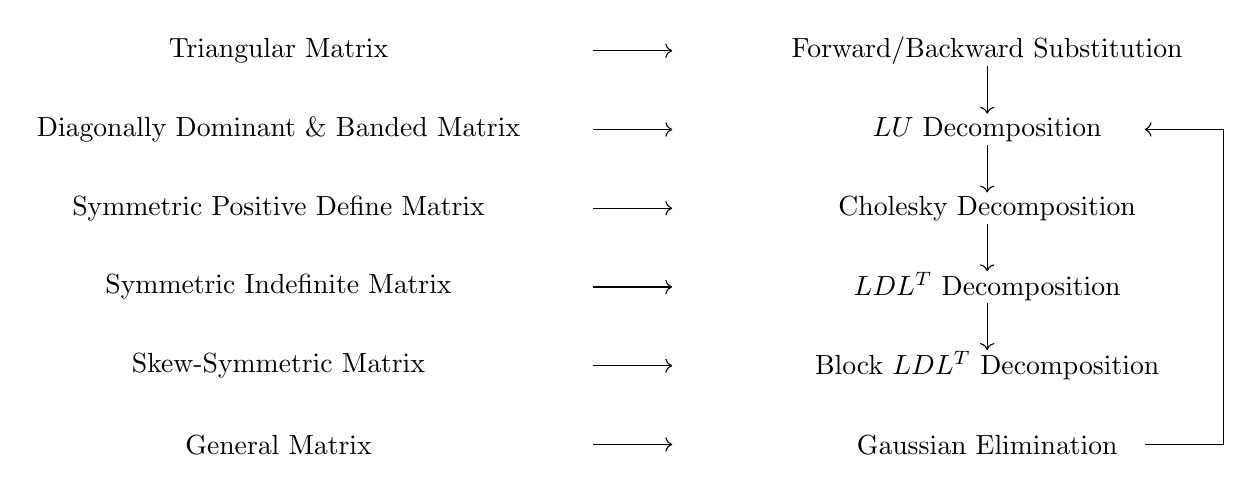
\begin{tikzpicture}
        \node at (0, 2) {Diagonally Dominant \& Banded Matrix};
        \node at (0, 3) {Triangular Matrix};
        \node at (0, 1) {Symmetric Positive Define Matrix};
        \node at (0, 0) {Symmetric Indefinite Matrix};
        \node at (0, -1) {Skew-Symmetric Matrix};
        \node at (0, -2) {General Matrix};
        \draw[->] (4, 2) -- (5, 2); \node at (9, 2) {$ LU $ Decomposition};
        \draw[->] (4, 3) -- (5, 3); \node at (9, 3) {Forward/Backward Substitution};
        \draw[->] (4, 1) -- (5, 1); \node at (9, 1) {Cholesky Decomposition};
        \draw[->] (4, 0) -- (5, 0); \node at (9, 0) {$ LDL^T $ Decomposition};
        \draw[->] (4, -1) -- (5, -1); \node at (9, -1) {Block $ LDL^T $ Decomposition};
        \draw[->] (4, -2) -- (5, -2); \node at (9, -2) {Gaussian Elimination};
        \draw[->] (9, 2.8) -- (9, 2.2);
        \draw[->] (9, 1.8) -- (9, 1.2);
        \draw[->] (9, 0.8) -- (9, 0.2);
        \draw[->] (9, -0.2) -- (9, -0.8);
        \draw[->] (11, -2) -- (12, -2) -- (12, 2) -- (11, 2);
      \end{tikzpicture}
    \caption{矩阵性质与相应方法}
    \label{fig:PropertyMethod}
\end{figure}
本文将先介绍最通用也最基础的高斯消元法,之后按从图\ref{fig:PropertyMethod}的上方到下方的顺序介绍这些方法,越上面的矩阵性质越好,对应的方法也越高效,但是适用性也越窄。在介绍每个方法时,将给出伪代码及其算法实现,并研究算法复杂度和稳定性。

\section{三角矩阵的直接解法}
这一节需要求解的问题形如$ Ux=b $,其中
\[
    U = \begin{pmatrix}
        u_{11} & u_{12} & \cdots & u_{1n} \\
        0 & u_{22} & \cdots & u_{2n} \\
        \vdots & \vdots & \ddots & \vdots \\
        0 & 0 & \cdots & u_{nn}
    \end{pmatrix}
\]
是任意的对角元非零上三角矩阵。
\subsection{后代法}
注意到解向量$ x $的第$ i $个分量$ x_i $满足
\[
    x_i = \frac{b_i - \sum_{j=i+1}^{n} u_{ij}x_j}{u_{ii}},
\]
在计算$ x_i $时只需要后$ n-i $个分量,而$ x_n = b_n / u_{nn} $,因此我们可以按照从后到前的顺序逐个计算$ x_i $。因为在计算每个$ x_i $时需要使用到$ U $的第$ i $行(row-oriented),因此这种方法称为\emph{行向}后代法,另外由于上式中的$ \sum_{j=i+1}^{n} u_{ij}x_j $可视作内积,因此该方法也称作\emph{内积型}(inner-product form)后代法。伪代码如算法\ref{alg:BackSub}所示,该算法有如下三点注意事项:
\begin{enumerate}
    \item 节省内存:注意到$ b_i $仅在计算$ x_i $时使用,因此可以直接在$ b $内储存每次计算得到的$ x_i $,最终$ b $即为解向量$ x $。
    \item 异常检验:如果$ u_{ii} = 0 $,则矩阵$ U $奇异,算法退出。
    \item 利用零元:如果右端项$ b $的末尾是一段长为$ l $的连续零元,则原问题退化为一个规模为$ n-l $的问题。
\end{enumerate}

\begin{algorithm}[htbp]
    \caption{Backward substitution (row-wise) for upper triangle matrix}\label{alg:BackSub}
    \KwData{$ U $ is a nonsingluar upper triangle matrix in $ \mathbb{R}^{n\times n} $,$ b $ is a vector in $ \mathbb{R}^n $.}
    \KwResult{$ x $ s.t. $ Ux=b $.}
    $ b_n = b_n/u_{nn} $\;
    \For{$ i = n-1:-1:1 $}{
        \For{$ j = i+1:n $}{
            $ b_i = b_i - u_{ij}b_j $       \tcc*[r]{Backward substitution}
        }
        \eIf{$ u_{ii} = 0 $}{
            \Return Matrix is singular, exit\;
        }
        {$ b_i = b/u_{ii} $\;}
    }
    \Return $ x=b $\;
    \KwCost{$ n(n-1)+n+n = O(n^2) $ flops.}
\end{algorithm}

除了行向后代法,还有一种\emph{列向}后代法,这种方法基于矩阵分块:将$ U $进行如下分块
\[
    U = 
    \begin{pmatrix}
        U' & u_{1:n-1,n}\\
        0 & u_{nn}
    \end{pmatrix},\quad
    U' = U(1:n-1,1:n-1),
\]
于是$ x_n = b_n / u_{nn} $,原问题$ Ux=b $转化为一个形式与原问题相同但维数低一维的问题
\[
    U'x' = b' - u_{1:n-1,n}x_n,
\]
因此这种方法可以递归实现。由于每次递归时需要使用到$ U $的一列,故称之为列向后代法。

对于下三角矩阵,相应的方法被称为前代法,类似地同样可以分为行向前代法和列向前代法,行向前代法的伪代码如\ref{alg:ForSub}所示。
\begin{algorithm}[htbp]
    \caption{Forward substitution (row-wise) for lower triangle matrix}\label{alg:ForSub}
    \KwData{$ L $ is a nonsingluar lower triangle matrix in $ \mathbb{R}^{n\times n} $,$ b $ is a vector in $ \mathbb{R}^n $.}
    \KwResult{$ x $ s.t. $ Lx=b $.}
    $ b_1 = b_1/l_{11} $\;
    \For{$ i = 2:n $}{
        \For{$ j = 1:i-1 $}{
            $ b_i = b_i - l_{ij}b_j $       \tcc*[r]{Forward substitution}
        }
        \eIf{$ l_{ii} = 0 $}{
            \Return Matrix is singular, exit\;
        }
        {$ b_i = b_i/l_{ii} $\;}
    }
    \Return $ x = b $\;
    \KwCost{$ n(n-1)+n+n = O(n^2) $ flops.}
\end{algorithm}

\subsection{误差分析}
这一小节我们将对上一小节给出的算法进行后向和前向误差分析,这些分析的基础是下面的引理,它刻画了浮点计算下后代或前代运算引入的误差。
\begin{lemma}\bf{\textup{后代运算}}
    如果$ x_i = (c_i - \sum_{j=i+1}^{n}x_{j} u_{ij})/u_{ii} $以
    \begin{verbatim}
        s = c(i)
        for j = i+1:n
            s = s - x(j) * u(i,j)
        end
        x = s / u(i,i)
    \end{verbatim}
    的方式进行浮点计算,则计算结果$ \hat{x}_i $满足
    \begin{equation}
        [u_{ii}(1+\theta_{n-i+1})] \hat{x}_i = b_i - \sum_{j=i+1}^{n} [u_{ij}(1+\theta_{j-i})]x_j,
    \end{equation}
    其中$ |\theta_j|\leqslant \gamma_j = ju / (1-ju) $。
\end{lemma}
因此根据上述引理,算法\ref{alg:BackSub}在浮点运算下得到的解向量$ \hat{x} $满足如下后向误差关系
\begin{equation}
    (U+\Delta U) \hat{x} = b,\quad 
    |\Delta u_{ij}| \leqslant 
    \begin{cases}
        \gamma_{n-i+1}|u_{ij}|, & i=j,\\
        \gamma_{|i-j|}|u_{ij}|, & i\ne j.
    \end{cases}
\end{equation}
类似地,对于前代运算$ x_i = (c_i - \sum_{j=1}^{i-1}x_{j} l_{ij})/l_{ii} $,如果按照类似引理中的顺序计算,则相应的浮点误差关系为
\begin{equation}
    [l_{ii}(1+\theta_{i})] \hat{x}_i = b_i - \sum_{j=1}^{i-1} [l_{ij}(1+\theta_{j})]x_j,
\end{equation}
因此算法\ref{alg:ForSub}在浮点运算下得到的解向量$ \hat{x} $满足如下后向误差关系
\begin{equation}
    (L+\Delta L) \hat{x} = b,\quad 
    |\Delta l_{ij}| \leqslant \gamma_j |l_{ij}|.
\end{equation}

实际上,无论计算使用的是什么顺序,对于后代法,我们都有
\[
    [u_{ii}(1+\theta^{(i)}_{n-i+1})] \hat{x}_i = b_i - \sum_{j=i+1}^{n} [u_{ij}(1+\theta^{(j)}_{n-i+1})]x_j,
\]
对于前代法,我们有
\[
    [l_{ii}(1+\theta_{i}^{(i)})] \hat{x}_i = b_i - \sum_{j=1}^{i-1} [l_{ij}(1+\theta_{i}^{(j)})]x_j,
\]
其中的$ \theta_{i}^{(j)}\leqslant \gamma_i $对任意$ j $都成立。于是无论是后代法还是前代法,我们都有如下后向误差关系
\begin{equation}
    \textcolor{red}{(T+\Delta T) \hat{x} = b,\quad
    |\Delta T|\leqslant \gamma_n |T|}.
\end{equation}

根据ASNA Th 7.4,我们知道在$ | \Delta A | \leqslant \epsilon E $,$ | \Delta b | \leqslant \epsilon f $,并且$ \epsilon\| |A^{-1}|E \|_\infty < 1 $时,前向误差满足
\begin{equation}
    \frac{\| x-y \|_\infty}{\| x \|_\infty} \leqslant \frac{\epsilon}{1-\epsilon \| |A^{-1}|E \|_\infty}  \frac{\| |A^{-1}|(E|x|+f) \|_\infty}{\| x \|_\infty },
\end{equation}
其中$ Ax=b $,$ (A+\Delta A)y = b + \Delta b $。而此时$ \epsilon = \gamma_n $,$ E = |T| $,$ f = 0 $,因此算法\ref{alg:BackSub}和算法\ref{alg:ForSub}的前向误差满足
\begin{equation}
    \frac{\| x-\hat{x} \|_\infty}{\| x \|_\infty} \leqslant \frac{\gamma_n}{1-\gamma_n \| |T^{-1}| |T| \|_\infty}  \frac{\| |T^{-1}||T|x| \|_\infty}{\| x \|_\infty }.
\end{equation}
注意到$ \| |T^{-1}| |T| \|_\infty = {\rm cond}(A) $,$ | |T^{-1}| |T| |x| \|_\infty / \| x \|_\infty = {\rm cond}(A,x) $分别是矩阵的Skeel条件数和线性系统的Skeel条件数,因此前向误差关系可以写为
\begin{equation}
    \textcolor{red}{\frac{\| x-\hat{x} \|_\infty}{\| x \|_\infty} \leqslant \frac{\gamma_n {\rm cond}(A,x)}{1-\gamma_n {\rm cond}(A)}}.
\end{equation}
考虑到由于
\[
    {\rm cond}(A) = \inf_D \kappa_\infty(DA),
\]
其中$ D $是任意非奇异对角矩阵,$ {\rm cond}(A) $可以比使用传统的$ \kappa_\infty(A) = \| A^{-1} \|_\infty \| A \|_\infty $给出更小的误差上界。另一方面,对于三角矩阵而言,病态性主要可能来自两个方面:一是各对角元之间的相对大小,二是非对角元与相应的该行或该列的对角元之间的相对大小。而Skeel条件数$ {\rm cond} $不同于传统条件数$ \kappa $,它在行放缩下保持不变$ {\rm cond}(DA) = {\rm cond}(A) $,因此只受到第二个方面的影响,故使用Skeel条件数在各方面均比传统条件数更为合适。不过,虽然$ {\rm cond}(T) $可能会远远小于$ \kappa_\infty(T) $,但是$ {\rm cond}(T,x) $可能仍然会非常大,好在对于一些特殊的三角矩阵,我们可以得到较好的前向误差估计。

\subsection{对角占优三角矩阵}
在各类算法中,对角占优的矩阵往往有比较好的性质,这一小节对于一些某种意义下的对角占优的三角矩阵给出了比之前更好的前向误差估计。

首先我们考虑对角元绝对值大于非对角元绝对值的三角矩阵,引理\ref{lem:DiagBig}给出了这类矩阵的Skeel条件数的上界,并且这一上界与条件数$ \kappa $无关,因此在行放缩下保持不变。
\begin{lemma}\label{lem:DiagBig}\bf{\textup{对角元绝对值大于非对角元绝对值}}
    如果上三角矩阵$ U\in \mathbb{R}^{n\times n} $满足如下条件:
    \begin{equation}
        |u_{ii}|\geqslant |u_{ij}|,\quad j>i,
    \end{equation}
    则单位对角上三角矩阵$ W = |U^{-1}| |U| $满足$ w_{ij}\leqslant 2^{j-i} $,进而我们有$ {\rm cond}(U) \leqslant 2^{n-1} $。
\end{lemma}
\noindent \emph{Hint:}注意到对于单位对角上三角矩阵$ V $,如果它的对角元绝对值大于非对角元绝对值,则任意$ j>i $都有$ |(V^{-1})_{ij}|\leqslant 2^{j-i-1} $。

根据之前的分析,后代法\ref{alg:BackSub}给出的计算结果$ \hat{x} $满足$ (U+\Delta U)\hat{x} = b $,于是
\[
    |x - \hat{x}| = |U^{-1} \Delta U \hat{x}|\leqslant |U^{-1}| |\Delta U| |\hat{x}|,
\]
又因为$ |\Delta U|\leqslant \gamma_n |U| $,所以
\[
    |x - \hat{x}| \leqslant \gamma_n |U| |U^{-1}| |\hat{x}|.
\]
所以如果$ U $满足引理\ref{lem:DiagBig}的条件,则
\[
    |x - \hat{x}| \leqslant \gamma_n W |\hat{x}|,
\]
展开右端矩阵乘法可以得到分量形式的前向误差估计
\begin{equation}\label{eq:DiagBig}
    |x_i - \hat{x}_i| \leqslant \gamma_n \sum_{j=i}^{n} w_{ij} |\hat{x}_j| \leqslant \gamma_n \sum_{j=i}^{n} 2^{j-i} \max_{k\geqslant i}|\hat{x}_k| \leqslant \textcolor{red}{2^{n-i+1}\gamma_n \max_{k\geqslant i}|\hat{x}_k|}.
\end{equation}
经过一些放缩也可以写成相对误差形式
\begin{equation}
    \frac{\| x - \hat{x} \|_\infty}{\| \hat{x} \|_\infty} \leqslant 2^{n} \gamma_n.
\end{equation}
根据(\ref{eq:DiagBig}),尽管在$ n $很大的时候前向误差界会很大,但是随着$ i $的增大,前向误差界会指数级减小,因此使用后代法计算这类矩阵的解时,靠后的分量的计算精度相比于靠前的分量会更高。

另外,对于下三角矩阵有类似的结论。不过,当上三角矩阵$ U $满足
\[
    |u_{ii}|\geqslant |u_{ij}|, \quad j>i,
\]
时,它的转置$ L = U^T $不一定满足
\[
    |l_{ii}|\geqslant |l_{ij}|, \quad j<i,
\]
这说明使用前代法和后代法求解系统$ Ly = c $的病态性与$ Ux = b $的病态性并非简单相同的。

对于要求更严格的对角占优矩阵,我们有更小的上界。
\begin{lemma}\label{lem:DiagDom}\bf{\textup{行对角占优三角矩阵}}
    如果上三角矩阵$ U\in \mathbb{R}^{n\times n} $满足如下条件:
    \begin{equation}
        |u_{ii}| \geqslant \sum_{j=i+1}^{n} |u_{ij}|,\quad i=1,2,\ldots,n,
    \end{equation}
    则称$ U $是行对角占优矩阵,并且单位对角上三角矩阵$ W = |U^{-1}| |U| $满足$ w_{ij}\leqslant i+j-1 $,进而我们有$ {\rm cond}(U) \leqslant 2n-1 $。
\end{lemma}
\noindent \emph{Hint:}注意到对于单位对角上三角矩阵$ V $,如果它是行对角占优的,则任意$ j>i $都有$ |(V^{-1})_{ij}|\leqslant 1 $,进而可得$ w_{ij}\leqslant i+j-1 $,于是
\[
    \| W \|_\infty = \| |W|e \|_\infty = \| |V^{-1}| |V| e \|_\infty \leqslant \| |V^{-1}| (2,2,\cdots ,2,1)^T \|_\infty \leqslant 2n-1.
\]

对于行对角占优三角矩阵,前向误差估计为
\begin{equation}
    |x_i - \hat{x}_i| \leqslant \gamma_n \sum_{j=i}^{n} w_{ij} |\hat{x}_j| \leqslant \gamma_n \sum_{j=i}^{n} (i+j-1) \max_{k\geqslant i}|\hat{x}_k| \leqslant \textcolor{red}{\frac{(n-i+1)(n+3i-2)}{2}\gamma_n \max_{k\geqslant i}|\hat{x}_k|}.
\end{equation}
这一上界远远小于对角元绝对值大于非对角元绝对值的三角矩阵的上界。

\subsection{并行算法}
这一节的最后我们给出求解三角矩阵的一种并行算法,该算法基于三角矩阵的矩阵分解。考虑下三角矩阵$ L $的如下分解
\[
    L = L_1 L_2 \cdots L_{n},
\]
其中
\[
    L_i =
    \begin{pmatrix}
        I_{i-1,i-1} & & & & \\
        & l_{ii} & & & \\
        & l_{i+1,i} & 1 & &\\
        & \vdots & & \ddots &\\
        & l_{ni} & & & 1
    \end{pmatrix}. 
\]
记$ M_i = L^{-1}_i $,于是线性方程组$ Lx=b $的解为
\begin{equation}
    x = M_n M_{n-1} \cdots M_1 b.
\end{equation}
在计算右端项时使用并行计算,如$ n=7 $时的计算过程如下
\[
    x = \{[(M_7M_6)(M_5M_4)][(M_3M_2)(M_1b)]\}.
\]
一般地,这种算法可以使用一棵深度为$ \lceil\log(n+1)\rceil +1 $的二分树来表示,一共需要$ O(n^3) $次运算,因此只适合使用并行计算。关于误差分析,这里只直接给出一些结论,细致的分析见ASNA sec 8.5。
计算结果$ \hat{x} $满足的后向误差公式为($ n=7 $)
\begin{equation}
    \hat{x} = \{[(M_7M_6+\Delta_{76})(M_5M_4+\Delta_{54})+\Delta_{7654}][(M_3M_2+\Delta_{32})(M_1+\Delta_1)b]\},
\end{equation}
相应的残差估计为
\begin{equation}
    \| b - L\hat{x} \|_\infty \leqslant d_n u \| |L| |L^{-1}| |L| |L^{-1}| |L| |x| \|_\infty + O(u^2),
\end{equation}
或者
\begin{equation}
    | b - L\hat{x} | \leqslant d_n u |L| |L^{-1}| |L| |L^{-1}| |L| |x|  + O(u^2),
\end{equation}
其中$ d_n = an\log n $,$ a = O(1) $。一般地,我们有后向误差关系
\begin{equation}
    (L+\Delta L) \hat{x} = b,\quad \| \Delta L \| \leqslant \alpha_n u \kappa_\infty(L)^2 \| L \|_\infty +O(u^2)
\end{equation}
其中$ \alpha_n = [n^2 \log n +O(n \log n)] / 2 $。前向误差估计为
\begin{equation}
    |x - \hat{x}| \leqslant  d_n' u M(L)^{-1}|b| + o(u^2),
\end{equation}
其中$ M(L) $是比较矩阵,即
\[
    (M(A))_{ij} = 
    \begin{cases}
        -|a_{ij}|, & i\ne j,\\
        |a_{ij}|, & i=j.
    \end{cases}
\]
上述估计也可以被放宽为
\begin{equation}
    \frac{\| x - \hat{x} \|_\infty}{\| x \|_\infty} \leqslant \frac{c_n u \| M(L)^{-1}|L| |x| \|_\infty}{\| x \|_\infty} + O(u^2),
\end{equation}
或者
\begin{equation}
    \frac{\| x - \hat{x} \|_\infty}{\| x \|_\infty} \leqslant \frac{d_n u \| (|L^{-1}| |L|)^3 |x| \|_\infty}{\| x \|_\infty } + O(u^2).
\end{equation}

\section{一般矩阵的Gauss消元法和LU分解}
Gauss消元法(GE)是求解线性方程组的最基础的直接法,它的基本思想是通过一系列的消元操作将系数矩阵化为上三角矩阵,然后使用上一节的方法求解上三角系统。
\subsection{原始Gauss消元法}
一般地,对于$ n $阶方阵,需要经过$ n $个阶段,从原本的$ A^{(1)} = A $,$ b^{(1)} = b $到最终的$ A^{(n)} = U $,$ b^{(n)} = A^{(n)}x $,在第$ k $个阶段,线性系统变为$ A^{(k)}x = b^{(k)} $,其中
\[
    A^{(k)} = 
    \begin{pmatrix}
        A^{(k)}_{11} & A^{(k)}_{12} \\
        0 & A^{(k)}_{22}
    \end{pmatrix},
\]
此处$ A^{(k)}_{11} $是一个$ k-1 $阶的上三角矩阵,而下一个阶段,即第$ k+1 $个阶段的操作则将使得$ A^{(k)}_{22} $的第一列除第一个元素外全部消为0,同时
\[
    \begin{aligned}
        a_{ij}^{(k+1)} &= a_{ij}^{(k)} - m_{ik} a_{kj}^{(k)},\quad i,j = k+1:n\\
        b_i^{(k+1)} &= b_i^{(k)} - m_{ik} b_k^{(k)},\quad i = k+1:n,
    \end{aligned}
\]
其中$ m_{ik} = a^{(k)}_{ik} / a^{(k)}_{kk} $。这一阶段需要$ 1+2(n-k)+2(n-k)^2 $,于是消元过程总的计算量为
\[
    \sum_{k=1}^{n-1} 1+2(n-k)+2(n-k)^2 = \frac{(2n-1)(n-1)n}{3}+n^2-1 = \frac{2}{3}n^3 + O(n^2),
\]
当使用后代法求解上三角系统时,计算量为$ O(n^2) $,因此不选主元的原始Gauss消元法的总计算量为$ O(n^3) $。

因为$ m_{ik} $与右端项$ b $无关,因此当$ b $发生改变时,每一步需要乘的因子$ m_{ik} $不会发生改变,所以储存$ m_{ik} $将使得Gauss消元在系数矩阵不变而右端项变化时无需重新进行对系数矩阵进行消元过程,只需改变右端项:
\[
    b_i^{(k+1)} = b_i^{(k)} - m_{ik} b_k^{(k)},\quad i = j+1:n, k=1:n-1,
\]
因此只需要$ O(n^2) $次运算,这大大节省了计算量。在上述操作中,由于在第$ k+1 $阶段,我们已经知道$ a^{(k+1)}_{ik} $全部变成了零元$ (i>k) $,因此没有必要储存这些零元,所以这些零元的位置正好可以用来储存$ m_{ik} $。注意到每一阶段的操作实际上等价于左乘一个矩阵$ M_k $,即
\[
    A^{(k+1)} = M_k A^{(k)},  
\]
其中
\[
    M_k =
    \begin{pmatrix}
        I_{k-1,k-1} & & & & \\
        & 1 & & & \\
        & -m_{k+1,k} & 1 & &\\
        & \vdots & & \ddots &\\
        & -m_{nk} & & & 1
    \end{pmatrix},
\]
所以我们有
\begin{equation}
    A^{(n)} = M_{n-1}M_{n-2}\cdots M_1 A = U,
\end{equation}
注意到下三角矩阵$ M_k $的逆同样是下三角矩阵
\[
    L_k = M_k^{-1} =
    \begin{pmatrix}
        I_{k-1,k-1} & & & & \\
        & 1 & & & \\
        & m_{k+1,k} & 1 & &\\
        & \vdots & & \ddots &\\
        & m_{nk} & & & 1
    \end{pmatrix},
\]
并且下三角矩阵的乘积仍然是下三角矩阵,因此我们有
\begin{equation}
    A = (L_{1}L_{2}\cdots L_{n-1})U = LU,
\end{equation}
这就是矩阵的LU分解,即
\begin{theorem}\label{thm:LU}\bf{\textup{LU分解}}
    \begin{enumerate}
        \item 如果$ n $阶方阵$ A $的各个顺序主子式非零,则$ A $可以进行LU分解,即存在唯一的单位下三角矩阵$ L $和上三角矩阵$ U $,使得$ A = LU $。
        \item 一个可逆矩阵可以进行LU分解的充要条件是它的所有子式都非零。
        \item 不可逆的矩阵也可能可以进行LU分解:任意秩为$ k $的矩阵如果前$ k $个顺序主子式非零,则它可以进行LU分解,否则不能进行LU分解。
    \end{enumerate}
\end{theorem}
\noindent 使用向量语言可以将如上推导成外积形式(Outer product form)。记$ \bm{m}_k = (0,\cdots ,0,m_{k+1,k},\cdots ,m_{n,k})^T $,则$ e_k^T \bm{m}_k=0 $而
\[
    \bm{m}_k  e_k^T = 
    \begin{pmatrix}
        0_{k-1,k-1} & & & & \\
        & 0 & & & \\
        & m_{k+1,k} & 0 & &\\
        & \vdots & & \ddots &\\
        & m_{nk} & & & 0
    \end{pmatrix},
\]
于是$ M_k = I - \bm{m}_k e_k^T $,而$ L_k = I + \bm{m}_k e^T_k $,故
\[
    L = \prod_{i=1}^{n-1}(I+\bm{m}_k e_k^T) = I + \sum_{i=1}^{n-1}\bm{m}_i e_i^T = 
    \begin{pmatrix}
        1 & & & & \\
        m_{21} & 1 & & & \\
        \vdots & \vdots & \ddots & &\\
        m_{n-1,1} & m_{n-1,2} & \cdots & 1 &\\
        m_{n1} & m_{n2} & \cdots & m_{n,n-1} & 1
    \end{pmatrix}.
\]

现在考虑LU分解的计算。为保证分解的唯一性,要求$ L $是单位对角的下三角矩阵($ l_{kk}=1 $),此时计算矩阵$ A\in \mathbb{R}^{m\times n} (m\geqslant n)$的LU分解等价于求解如下问题:
\begin{equation}
    a_{ij} = \sum_{r=1}^{\min(i,j)} l_{ir} u_{rj}.
\end{equation}
于是
\[
    \begin{aligned}
        a_{kj} &= l_{k1}u_{1 j}+\cdots +l_{k,k-1}u_{k-1,j}+ \boxed{\textcolor{blue}{u_{kj}}},\quad j=k:n,\\
        a_{ik} &= l_{i1}u_{1 k}+\cdots +l_{i,i-1}u_{i-1,k}+ \boxed{\textcolor{blue}{l_{ik}}}u_{kk},\quad i=k+1:m,
    \end{aligned}
\]
根据第一个公式先得到$ U $的第$ k $行元素,再带入第二个公式可得$ L $的第$ k $列元素,该过程称为计算LU分解的\emph{Doolittle方法},具体算法见\ref{alg:Doolittle},该算法等价于进行原始Gauss消元过程(储存消元因子$ m_{ik} $),从上到下从左到右使用$ A $中的各元素。当要求$ U $是单位对角的上三角矩阵时,有类似的\emph{Crout方法},这种情况下需要先计算$ L $的第$ k $列元素后再带入$ U $的第$ k $行元素。

\begin{algorithm}[htbp]
    \caption{Doolittle's method}\label{alg:Doolittle}
    \KwData{$ A\in \mathbb{R}^{m\times n}(m\geqslant n) $.}
    \KwResult{Unit lower triangle matrix $ L $ and upper triangle matrix $ U $ s.t. $ A = LU $.}
    \For{$ k = 1:n $}{
        \tcc{Compute $ U $'s $ k $-th row}
        \For{$ j = k:n $}{
            $ u_{kj} = a_{kj} - \sum_{i=1}^{k-1}l_{ki}u_{ij} $       \tcc*[r]{Inner-product form}
        }
        \tcc{Compute $ L $'s $ k $-th column}
        \For{$ i = k+1:m $}{
            $ l_{ik} = (a_{ik} - \sum_{j=1}^{k-1}l_{ij}u_{jk}) / u_{kk} $       \tcc*[r]{Inner-product form}
        }
    }
    \Return $ L,U $\;
    \KwCost{$ mn^2-n^3 / 3-n^2 / 2 - n / 6 =  O(n^2(m- n /3)) $ flops.}
\end{algorithm}

\subsection{选取主元——Pivoting}
原始的Gauss消元法具有以下几点缺点:
\begin{itemize}
    \item $ a_{kk}^{(k)} = 0 $时出现除零操作,算法中断;
    \item $ m_{ik} $过大时,计算$ a_{ij}^{(k)} - m_{ik}a^{(k)}_{kj} $中的减法时会丢失一些准确位数(大数吃小数),这部分精度的丢失可能会导致最终矩阵相对于原矩阵而言出现较大的差异;
    \item 要求$ A $的各个顺序主子式非零,该条件过于苛刻。
\end{itemize}
本小节我们将讨论如何通过选取主元来解决上述问题。

不难发现,前两个问题的根源在于$ a_{kk}^{(k)} $(\emph{主元})太小,在消元时我们又需要计算一次除法$ m_{ik} = a_{ik}^{(k)} / a_{kk}^{(k)} $,而在数值计算中我们应当尽量避免出现一个微小的数做除数。为了修复前两个问题,一种自然的想法是在第$ k $个阶段通过行变换或列变换(或者两者兼有)将别的元素调到$ a_{kk}^{(k)} $的位置,即线性系统的重新排列,使得新的$ a_{kk}^{(k)} $相对更好。这种方法称为\emph{选取主元}。一般地,选取主元的方法有以下几种:
\begin{itemize}
    \item \emph{部分主元策略}:在第$ k $个阶段,选取$ a_{kk}^{(k)} $所在列的位于$ a_{kk}^{(k)} $及其下方的绝对值最大的元素作为主元,即若
    \[
        |a_{rk}^{(k)}| = \max_{k\leqslant i\leqslant n} |a_{ik}^{(k)}|,
    \]
    则交换第$ k $行与第$ r $行,使用原本的$ |a_{rk}^{(k)}| $作为该阶段的主元,这将保证$ |m_{ik}|\leqslant 1 $,其中$ i\leqslant n $。部分策略需要$ O(n^2) $次比较确定新的主元。
    \item \emph{完全主元策略}:在第$ k $个阶段,选取子矩阵$ A^{(k)}(k:n,k:n) $中绝对值最大的元素作为主元,即
    \[
        |a_{rs}^{(k)}| = \max_{k\leqslant i,j\leqslant n} |a_{ij}^{(k)}|,
    \]
    则先交换第$ k $行与第$ r $行,再交换第第$ k $行与第$ s $行,使用原本的$ |a_{rs}^{(k)}| $作为该阶段的主元,同样$ |m_{ik}|\leqslant 1 $,其中$ i\leqslant n $。这种策略为了确定新的主元需要$ O(n^3) $次比较。
    \item \emph{Rook 策略}:该策略是前两种策略的折中,因为选主元的轨迹类似于象棋中车的走法,故称为Rook策略。该策略同时进行列搜索和行搜索,每次搜索时选取绝对值最大的元素作为主元,直到某一步的元素同时是行最大和列最大的元素,这时选取该元素作为主元。这种策略在最坏情况下也可能需要$ O(n^3) $次比较,不过在实际对于大多数矩阵而言,rook策略所需的比较次数通常是部分主元策略的某几倍,但是远远小于完全主元策略。
\end{itemize}

至于第三个问题,事实上,当$ A $的某个顺序主子式为零时,理论上来讲对于欠定系统仍然可能有解,因此通过(完全或Rook)选取主元可以避免出现除零操作,于是LU分解仍然存在,但是不再唯一。这一事实再次体现了选主元的必要性。另一方面,在实际计算中,由于舍入误差的存在,无法准确判断一个数是否为零,因此在任何情况下,我们都应当通过选主元的方法尽量避免出现一个小数做除数的情况。同时,为了在系统可能是奇异时给出警告,我们应当在选取主元之后检查最终的主元是否足够小,若小于某个阈值则警告该系统可能接近奇异,因为
\[
    {\rm Rank} \begin{pmatrix}
        A_{11} & A_{12} \\
        0 & A_{22}
    \end{pmatrix} \leqslant {\rm Rank} (A_{11}) + {\rm Rank} (A_{22}),
\]
当最终的主元接近零时,说明真实的$ {\rm Rank} (A_{22}) $可能不满秩,如果$ {\rm Rank} (A_{22}) $不满秩则原矩阵奇异。

原始Gauss消元法等价于对$ A $进行LU分解的同时对$ b $做相应的行变换,而选取主元的Gauss消元法则对应于对经过了一些行交换和列交换之后的$ A $进行LU分解,选取主元后消元得到的$ A^{(k+1)} $此时满足
\[
    A^{(k+1)} = 
    \begin{cases}
        M_kP_kA^{(k)},& \text{Partial pivoting},\\
        M_kP_kA^{(k)}Q_k,& \text{Complete pivoting},
    \end{cases}
\]
其中$ P_k,Q_k $是置换矩阵(逆是自身),因此对于部分主元策略(GEPP),我们有
\[
    \begin{aligned}
        A^{(n)} = U 
        &= M_{n-1}(P_{n-1}M_{n-2}P_{n-1})\cdots (P_{n-1}\cdots P_{i+1}M_{i}P_{i+1}\cdots P_{n-1})\cdots (P_{n-1}\cdots P_1A)\\
        &= M_{n-1}'M_{n-2}'\cdots M_1'PA,
    \end{aligned}
\]
其中
\[
    M_{i}' = P_{n-1}\cdots P_{i+1}M_{i}P_{i+1}\cdots P_{n-1},\quad P = P_{n-1}\cdots P_1.
\]
因为$ M_i = I - \bm{m}_i e_i^T $,所以
\[
    M_i' = I - (P_{n-1}\cdots P_{i+1} \bm{m}_i)e_i^T
\]
是下三角矩阵,于是记$ L_i = (M_i')^{-1} $,$ L = L_1 L_2\cdots L_{n-1} $,则
\begin{equation}
    PA = LU,
\end{equation}
这种分解称为PLU分解。类似地,对于完全主元策略和Rook策略,我们有
\begin{equation}
    PAQ = LU.
\end{equation}

\subsection{误差分析}
由于选取主元的GE等价于先对矩阵重新排列再进行原始GE,因此在进行误差分析时只需考虑不选主元的原始Gauss消元法即可。另一方面,由于在GE的各种实现中,核心的步骤都是计算内积以及回代,所以它们的误差分析都是相似的,事实上,所有的这些实现都满足同一个误差界(如果不特别优化求和和内积运算),因此我们只需要分析Doolittle方法这一种简单实现的误差即可。

根据之前关于内积的分析,在Doolittle方法\ref{alg:Doolittle}中的两个内积计算的误差界满足
\[
    \begin{aligned}
        \left\vert a_{ik} - \sum_{j=1}^{k}\hat{l}_{ij} \hat{u}_{jk} \right\vert &\leqslant \gamma_k \sum_{j=1}^k |\hat{l}_{ij}| |\hat{u}_{jk}|,\quad i>k,\\
        \left\vert a_{kj} - \sum_{i=1}^{k-1}\hat{l}_{ki} \hat{u}_{ij} - \hat{u}_{kj} \right\vert &\leqslant \gamma_k \sum_{i=1}^k |\hat{l}_{ki}| |\hat{u}_{ij}|,\quad j\geqslant k.
    \end{aligned}
\]
因此LU分解的后向误差关系为
\begin{equation}
    \textcolor{red}{\hat{L} \hat{U} = A + \Delta A, \quad |\Delta A| \leqslant \gamma_n |\hat{L}| |\hat{U}|},
\end{equation}
得到了LU分解之后,需要依次求解两个三角系统
\[
    \hat{L} y = b, \quad \hat{U} x = y,
\]
通过前代法和后代法求解这两个系统的误差关系为
\[
    \begin{aligned}
        (\hat{L}+\Delta L) \hat{y} = b, \quad |\Delta L| \leqslant \gamma_{n} |\hat{L}|,\\
        (\hat{U}+\Delta U) \hat{x} = \hat{y}, \quad |\Delta U| \leqslant \gamma_{n} |\hat{U}|,
    \end{aligned}
\]
所以总的来说,使用GE求解线性系统的后向误差关系为
\begin{equation}\label{eq:GEbackerror}
    \textcolor{red}{(A + \Delta A) \hat{x} = b, \quad |\Delta A| \leqslant \gamma_{3n} |\hat{L}| |\hat{U}|},
\end{equation}
其中
\[
    \Delta A = (\hat{L} \hat{U}-A) + \hat{L} \Delta U + \Delta L \hat{U} + \Delta L \Delta U,
\]
所以满足
\[
    |\Delta A| \leqslant  |\hat{L} \hat{U}-A| + |\hat{L} \Delta U| + |\Delta L \hat{U}| + |\Delta L \Delta U| \leqslant (3\gamma_{n} + \gamma_n^2) |\hat{L}| |\hat{U}|.
\]

这一后向误差关系看上去并不令人满意,我们通常希望扰动矩阵$ \Delta A $可以被形如$ E = F(A) $形式的矩阵所控制,这样方便我们使用条件数来估计前向误差并分析系统的稳定性,而不是像现在一样只得到了$ \Delta A $和$ |\hat{L}| |\hat{U}| $之间的关系。然而,这一关系是目前我们所能期望最好的结果,因为如果要分析$ \hat{L} $和$ \hat{U} $与$ A $之间的联系的话,因为消元过程中每一阶段的状态取决于上一阶段的情况,所以我们需要考虑所有的消元过程,这将使得分析变得非常困难复杂的同时也难以获得简洁的结果。不过,在一些特殊情况下,如果矩阵$ A $具有一些特殊的结构,我们可以通过分析这些结构来相对容易地给出$ \Delta A $与$ A $之间的联系。最简单地,当$ |\hat{L}| |\hat{U}|=|\hat{L} \hat{U}| $时,我们有
\[
    |\hat{L}| |\hat{U}| = |\hat{L} \hat{U}| = |A+\Delta A| \leqslant |A| + \gamma_n |\hat{L}| |\hat{U}|,
\]
于是
\[
    |\hat{L}| |\hat{U}| \leqslant \frac{|A|}{1-\gamma_n},
\]
进而使用$ \Delta A $和$ |\hat{L}| |\hat{U}| $之间的关系和上述不等式可得
\begin{equation}
    (A+\Delta A) \hat{x} = b,\quad |\Delta A| \leqslant \frac{\gamma_{3n}}{1-\gamma_n}|A|.
\end{equation}

显然当$ |\hat{L}|$和$|\hat{U}| $均非负时条件$ |\hat{L}| |\hat{U}|=|\hat{L} \hat{U}| $可以满足,而有一类被称为\emph{完全非负矩阵}的矩阵,这些矩阵的LU分解可以证明都是非负的,故满足这一条件。如果某个矩阵的各个子式全都非负,则就称它是完全非负的。如果把条件严格到矩阵的各个子式都是正的,则相应的LU分解的各元不仅是严格正的而且距离零将足够远,另外对这类矩阵而言无需进行选主元,可以证明不选主元等价于完全主元策略。

现在回到后向误差估计(\ref{eq:GEbackerror}),将该式与$ Ax=b $相见可得
\[
    |\hat{x} - x| = |A^{-1} \Delta A \hat{x}|\leqslant \gamma_{3n} | A^{-1} | |\hat{L}| |\hat{U}| | \hat{x} - x |,
\]
因此前向误差关系为
\begin{equation}
    \textcolor{red}{\frac{\| x - \hat{x} \|_\infty}{\| x \|_\infty} \leqslant \gamma_{3n}  \frac{\| | A^{-1} | | \hat{L} | |\hat{U}| |\hat{x}| \|_\infty}{\| x \|_\infty}},
\end{equation}
再使用一次范数的一致性可得
\begin{equation}
    \frac{\| x - \hat{x} \|_\infty}{\| x \|_\infty} \leqslant \gamma_{3n}\kappa_\infty  \frac{\| | \hat{L} | |\hat{U}| \|_\infty}{\| A \|_\infty}.
\end{equation}
如之前所说,这一误差界中$ |\hat{L}| |\hat{U}| $不直接与$ A $相关使得进一步分析比较困难,不过这里我们使用一些技巧可以把$ \hat{L} $给消去,并使用Skeel条件数给出上界。注意到LU分解满足
\[
    \hat{L} \hat{U} = A + \Delta A_0,\quad |\Delta A_0|\leqslant \gamma_n |\hat{L}| |\hat{U}|,
\]
因此$ \hat{L} = (A+\Delta A_0)\hat{U}^{-1} $,于是
\[
    |\hat{L}| |\hat{U}| \leqslant |(A+\Delta A_0)\hat{U}^{-1}| |\hat{U}|\leqslant (|A|+\gamma_n|\hat{L}| |\hat{U}|)|\hat{U}^{-1}| |\hat{U}|,
\]
移项可得
\[
    |\hat{L}| |\hat{U}|\leqslant |A| |\hat{U}^{-1}| |\hat{U}| (I - \gamma_n |\hat{U}^{-1}| |\hat{U}|)^{-1}.
\]
所以(\ref{eq:GEbackerror})中的$ \Delta A $满足
\begin{equation}
    |\Delta A| \leqslant  \gamma_{3n}|\hat{L}| |\hat{U}|\leqslant \gamma_{3n}|A| |\hat{U}^{-1}| |\hat{U}| (I - \gamma_n |\hat{U}^{-1}| |\hat{U}|)^{-1}.
\end{equation}
进而
\[
    |\hat{x} - x| = |A^{-1} \Delta A \hat{x}|\leqslant \gamma_{3n} | A^{-1} | |A| |\hat{U}^{-1}| |\hat{U}| (I - \gamma_n |\hat{U}^{-1}| |\hat{U}|)^{-1}|\hat{x}|,
\]
所以可得分量意义下的前向误差关系为
\begin{equation}
    \begin{aligned}
        \frac{\| x - \hat{x} \|_\infty}{\| x \|_\infty} &\leqslant 3nu \frac{\| | A^{-1} | | A | |\hat{U}^{-1}| |\hat{U}| |\hat{x}| \|_\infty}{\| x \|_\infty} + O(u^2)\\
        &\leqslant \textcolor{red}{3n u {\rm cond}(A) {\rm cond}(U)+O(u^2)}.
    \end{aligned}
\end{equation}
其中$ {\rm cond}(U) $在使用完全主元策略或Rook策略时满足$ {\rm cond}(U)\leqslant 2^n-1 $,当对于行对角占优矩阵使用原始GE时满足$ {\rm cond}(U)\leqslant 2n-1 $。不过$ {\rm cond}(U) $没有一般性的上界。

\subsection{增长因子}
尽管无法直接给出$ \Delta A $与$ A $之间的联系,我们还是希望对GE的数值稳定性进行一些定量分析,为此我们引入增长因子来对Gauss消元法进行后向误差分析,它使得我们可以相对粗略地估计$ L $和$ U $与$ A $之间的大小关系。定义矩阵$ A $的\emph{增长因子}为
\begin{equation}
    \rho_n = \frac{\max\limits_{i,j,k}|a_{ij}^{(k)}|}{\max\limits_{i,j}|a_{ij}|}.
\end{equation}
注意到$ A^{(n)} = U $,所以
\[
    u_{ij} = a_{ij}^{(n)} \leqslant \rho_n \max_{i,j}|a_{ij}|,
\]
由此我们有如下结果。

\begin{theorem}
    在GE过程中获得的矩阵$ A $的LU分解$ A = LU $(准确结果)满足
    \begin{equation}
        \| |L| |U|  \|_\infty \leqslant [1+2(n^2-n)\rho_n] \| A \|_\infty.
    \end{equation}
    使用GEPP求解线性系统$ Ax=b $得到的数值解$ \hat{x} $满足如下后向误差关系(Wilkinson)
    \begin{equation}
        (A+\Delta A)\hat{x} = b,\quad \textcolor{red}{\| \Delta A \|_\infty \leqslant n^2 \gamma_{3n} \rho_n \| A \|_\infty}.
    \end{equation}
\end{theorem}
\noindent \emph{Hint:}为了得到第二个公式中,实际上我们含糊使用了$ \hat{u}\leqslant \rho_n \max_{i,j}|a_{ij}| $而非根据定义的$ u\leqslant \rho_n \max_{i,j}|a_{ij}| $,不过考虑到这只是一个粗略的估计,所以在这里我们就先止步于此。而第一个结果的证明需要注意到
\[
    \textcolor{blue}{\tilde{A}^{(k+1)} = \tilde{A}^{(k)} - \bm{l}_k \bm{u}_k^T},
\]
其中$ \tilde{A}^{(k)} $与$ A^{(k)} $的区别仅在于$ \tilde{A}^{(k)} $的前$ k-1 $行都是$ 0 $,而$ \bm{l}_j $是$ L $的第$ j $列,$ \bm{u}_i $是$ U $的第$ i $行。于是
\[
    |\bm{l}_k| |\bm{u}_k|^T \leqslant |\tilde{A}^{(k)}| + |\tilde{A}^{(k+1)}|,
\]
而
\[
    |L| |U| = \sum_{i=1}^n |\bm{l}_i| |\bm{u}_i|^T.
\]

可以证明对于部分主元策略,增长因子$ \rho^p_n $具有上界$ 2^{n-1} $,并且$ \rho^p_n = 2^{n-1} $的矩阵都形如
\[
    DM \begin{pmatrix}
        T & \vdots & \alpha d\\
        0 & \vdots & \\
    \end{pmatrix},
\]
其中$ D = \operatorname{diag}(\pm 1) $,$ M $是单位对角下三角矩阵并且满足$ m_{ij} = -1\ (i>j) $,$ T $是任意$ n-1 $阶非奇异上三角矩阵,$ d = (1,2,\cdots ,2^{n-1})^T $,$ \alpha = |a_{1n}| = \max_{ij}|a_{ij}| $。不过,尽管这种增长因子以指数级增长的矩阵存在,但是在实际计算中,部分主元策略的增长因子通常是一个较小的常数。

而对于完全主元策略,Wilkinson证明了
\begin{equation}
    \rho^c_n \leqslant \sqrt{n(2\cdot 3^{1 / 2}\cdots n^{1 / (n-1)})} \sim cn^{1/2 +(\log n) / 4},
\end{equation}
并且右端的上界无法达到。

最后,Foster证明Rook策略下的增长因子$ \rho^r_n $满足
\begin{equation}
    \rho^r_n \leqslant \frac{3}{2}n^{\frac{3}{4}\log n}.
\end{equation}
\begin{figure}[htpb]
    \centering
    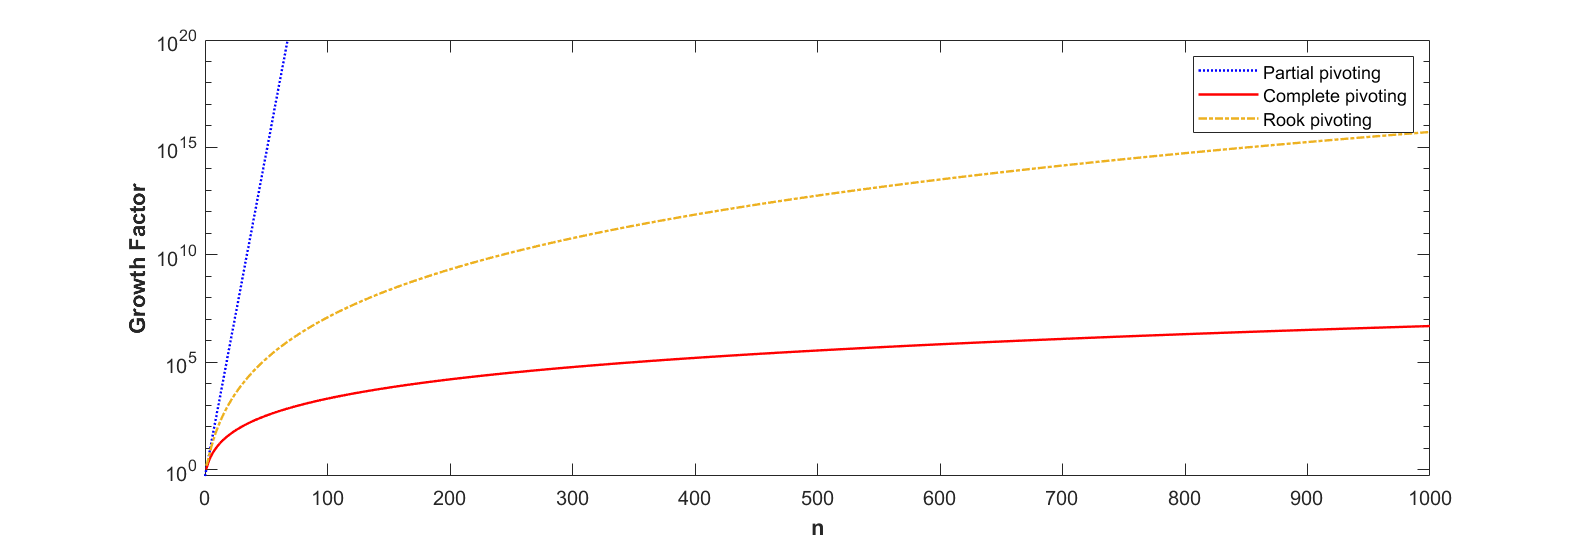
\includegraphics[width=0.8\textwidth]{GrowthFactor.png}
    \caption{三种策略的增长因子上界}\label{fig:GrowthFactor}
\end{figure}

对于一些特殊矩阵,增长因子可以给出足够好的上界。
\subsubsection{对角占优矩阵}
如果矩阵$ A\in \mathbb{C}^{n\times n} $满足
\[
    |a_{ii}| \geqslant \sum_{j\neq i} |a_{ij}|,\quad i=1:n,
\]
则称该矩阵是行对角占优矩阵。类似地,如果
\[
    |a_{ii}| \geqslant \sum_{j\neq i} |a_{ji}|,\quad i=1:n,
\]
则称该矩阵是列对角占优矩阵。如果上述条件中的“$ \geqslant $”变为“$ > $”,则称为强行对角占优或强列对角占优,这类矩阵是非奇异的。很多从有限元方法得到的矩阵都是对角占优的。对行或列对角占优矩阵,我们有如下结论。
\begin{theorem}
    如果$ A $是非奇异的行或列对角占优矩阵,则$ A $的LU分解存在并可以通过GE过程获得,且不选主元的GE增长因子满足
    \begin{equation}
        \rho_n \leqslant 2.
    \end{equation}
    另外,如果$ A $是列对角占优矩阵,则通过GE获得的LU分解中的$ l_{ij}\leqslant 1 $,因此对这类矩阵而言GEPP等价于GE。
\end{theorem}
事实上,根据引理\ref{lem:DiagDom}我们有
\[
    {\rm cond}(U) = \| |U^{-1}| |U| \|_\infty \leqslant 2n-1,
\]
而注意到
\[
    |L| |U| = |A U^{-1}| |U| \leqslant |A| |U^{-1}| |U|,
\]
于是
\[
    \| |L| |U| \|_\infty \leqslant {\rm cond}(U)\| A \|_\infty = (2n-1)\| A \|_\infty.
\]
所以尽管$ L $内的$ m_{ij} $可能很大,但是$ U $内的相应的$ u_{ij} $足够小,使得$ |L| |U| $的大小可以较好地被控制。根据(\ref{eq:GEbackerror}),对一般的矩阵进行GE的后向误差满足
\[
    (A + \Delta A) \hat{x} = b, \quad |\Delta A| \leqslant \gamma_{3n} |\hat{L}| |\hat{U}|
\]
因此对于对角占优矩阵,我们有
\[
    \| \Delta A \|_\infty \leqslant \gamma_{3n} \| |\hat{L}| |\hat{U}| \|_\infty\lesssim (2n-1)\gamma_{3n} \| A \|_\infty,
\]
所以这种情况下原始Gauss消元法是后向稳定的。

\subsubsection{带状矩阵}
\begin{figure}[htpb]
    \centering
    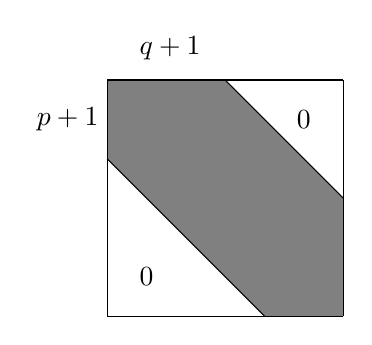
\begin{tikzpicture}
        \fill[gray] (0,2) -- (2,0) -- (3,0) -- (3,1.5) -- (1.5, 3) -- (0,3) -- cycle;
        \draw[-] (0, 0) -- (0, 3);
        \draw[-] (0, 0) -- (3, 0);
        \draw[-] (0, 3) -- (3, 3);
        \draw[-] (3, 0) -- (3, 3);
        \draw[-] (0, 2) -- (2, 0);
        \draw[-] (1.5, 3) -- (3, 1.5);
        \node[] at (2.5, 2.5) {$ 0 $};
        \node[] at (0.5, 0.5) {$ 0 $};
        \node[] at (-0.5, 2.5) {$ p+1 $};
        \node[] at (0.8, 3.4) {$ q+1 $};
      \end{tikzpicture}
    \caption{带状矩阵}
    \label{fig:BandMatrix}
\end{figure}
如图\ref{fig:BandMatrix}所示,如果矩阵$ A\in \mathbb{C}^{n\times n} $满足
\begin{equation}
    a_{ij} = 0, \quad i-j>p \text{ or } j-i>q,
\end{equation}
则称该矩阵是带状矩阵,其中$ p $和$ q $分别称为上带宽和下带宽。对于带状矩阵,我们有如下结论。
\begin{theorem}
    如果$ A $是上下带宽分别为$ p,q $的带状矩阵,则使用GEPP得到的LU分解$ PA = LU $中,$ L $的每列最多有$ p+1 $个非零元,$ U $的上带宽为$ p+q $。并且部分主元的GE增长因子满足
    \begin{equation}
        \rho_n^p \leqslant 2^{2p-1} - (p-1)2^{p-2},
    \end{equation}
    并且右端上界在$ n=2p+1 $时几乎达到。
\end{theorem}

在QR算法中起重要作用的上Hessenberg矩阵($ i-j>1 $时$ a_{ij} = 0 $)是一类特殊的带状矩阵,它在部分主元策略的GE的增长因子满足
\[
    \rho_n^p \leqslant n.
\]

另一类重要的带状矩阵是三对角矩阵,即
\[
    A = 
    \begin{pmatrix}
        d_1 & e_1 & & & \\
        c_2 & d_2 & e_2 & & \\
        & c_3 & d_3 & \ddots & \\
        & & \ddots & \ddots & e_{n-1} \\
        & & & c_{n} & d_n
    \end{pmatrix}.
\]
它的LU分解$ A = LU $形如
\[
    L = 
    \begin{pmatrix}
        1 & & & & \\
        l_2 & 1 & & & \\
        & l_3 & 1 & & \\
        & & \ddots & \ddots & \\
        & & & l_n & 1
    \end{pmatrix},\quad U =
    \begin{pmatrix}
        u_1 & e_1 & & & \\
        & u_2 & e_2 & & \\
        & & \ddots & \ddots & \\
        & & & \ddots & e_{n-1} \\
        & & & &  u_n
    \end{pmatrix},
\]
消元过程简化为$ u_1 = d_1 $,以及
\[
    \begin{aligned}
        l_i &= c_i / u_{i-1},\quad i=2:n,\\
        u_i &= d_i - l_i e_{i-1},\quad i=2:n.
    \end{aligned}
\]
所以计算结果满足
\[
    \begin{aligned}
        (1+\epsilon_i)\hat{l}_i &= c_i / \hat{u}_{i-1},\quad |\epsilon_i|\leqslant u\\
        (1+\theta_i)\hat{u}_i &= d_i - \hat{l}_i e_{i-1}(1+\delta_i),\quad |\theta_i|,|\delta_i|\leqslant u.
    \end{aligned}  
\]
于是
\[
    \begin{aligned}
        |c_i - \hat{l}_i \hat{u}_{i-1}| &\leqslant  u(\hat{l}_i \hat{u}_{i-1}),\\
        |d_i - \hat{u}_i - \hat{l}_ie_{i-1}| &\leqslant  u(|\hat{l}_{i} e_{i-1} +|\hat{u}_{i}|).
    \end{aligned}
\]
即
\begin{equation}
    A - \hat{L} \hat{U} = \Delta A, \quad |\Delta A| \leqslant u|\hat{L}| |\hat{U}|.
\end{equation}
使用回代法计算引入的误差满足
\begin{equation}
    (\hat{L}+\Delta L)(\hat{U} + \Delta U)\hat{x} = b,\quad |\Delta L|\leqslant u|\hat{L}|,|\Delta U| \leqslant (2u+u^2)|\hat{U}|,
\end{equation}
因此最终的后向误差满足
\begin{equation}
    (A+\Delta A)\hat{x} = b,\quad |\Delta A| \leqslant (4u+3u^2+u^3)|\hat{L}| |\hat{U}|.
\end{equation}

有几类特殊的三对角矩阵满足之前的$ |L| |U| = |LU| $的条件,这些矩阵的LU分解的增长因子可以给出较好的上界。
\begin{theorem}
    如果非奇异的三对角矩阵$ A $可以进行LU分解并且满足以下条件之一:
    \begin{enumerate}
        \item $ A $是对称正定的;
        \item $ A $是完全非负的,或等价地存在$ L\geqslant 0,U\geqslant 0 $使得$ A=LU $;
        \item $ A $是M-矩阵,即$ L $和$ U $的对角元都是正的,且非对角元非负;
        \item $ A = D_1BD_2 $,其中$ B $是满足之前条件之一的矩阵,$ |D_1|=|D_2|=I $是符号矩阵;
    \end{enumerate}
    则$ A $的LU分解满足$ |L| |U| = |LU| $。并且当$ A $是以上四类矩阵之一时,如果单位舍入误差$ u $足够小,则Gauss消元得到的数值解$ \hat{x} $满足如下后向误差关系:
    \begin{equation}
        (A+\Delta A)\hat{x} = b,\quad |\Delta A| \leqslant \frac{4u+3u^2+u^3}{1-u}|A|.
    \end{equation}
\end{theorem}

另外,如果矩阵$ A $是三对角矩阵但不属于上述定理中的四类矩阵之一,而只是行或列对角占优的,则虽然此时$ |L| |U| $可能不和$ |LU|=|A| $相同,但是$ |L| |U| $的大小仍然可以被控制,我们有
\[
    |L| |U| \leqslant 3|A|.
\]

\subsection{LU分解的稳定性}
这一节的最后,我们回过来考虑LU分解的敏感性问题,之前已经给出了LU分解的后向误差关系:
\[
    \hat{L} \hat{U} = A + \Delta A,\quad |\Delta A| \leqslant \gamma_{n} |\hat{L}| |\hat{U}|,
\]
但没有给出前向误差估计。尽管对于大多数应用而言,LU分解的前向误差分析不像后向误差分析那样重要,在这里我们还是给出一个简单的前向误差估计(ANSA Th 9.15)。
\begin{theorem}
    如果$ A\in \mathbb{R}^{n\times n} $非奇异,扰动后的$ A+\Delta A $也可逆,并且两者都有LU分解:
    \[
        A = LU, \quad A+\Delta A = (L+\Delta L)(U +\Delta U).
    \]
    令$ G = L^{-1}\Delta A U^{-1} $,则在$ \| G \|_2 $时,LU分解的前向误差满足
    \begin{equation}
        \max\left\{ \frac{\| \Delta L \|_F }{\| L \|_2}, \frac{\| \Delta U \|_F }{\| U \|_2} \right\} 
        \leqslant \frac{\| G \|_F}{1-\| G \|_2}\leqslant 
        \frac{\| L^{-1} \|_2 \| U^{-1} \|_2 \| A \|_2}{1-\| L^{-1} \|_2 \| U^{-1} \|_2 \| \Delta A \|_2} \cdot \frac{\| \Delta A \|_F}{\| A \|_F}.
    \end{equation}
    另外记$ \tilde{G} = (L+\Delta L)^{-1} \Delta A (U+\Delta U)^{-1} $,如果$ |\tilde{G}| $的谱半径(最大绝对值的特征值)小于$ 1 $,则有
    \begin{equation}
        \begin{aligned}
            |\Delta L|&\leqslant |L+\Delta L|\cdot {\rm stril}((I-|\tilde{G}|)^{-1}|\tilde{G}|),\\
            |\Delta U|&\leqslant {\rm triu}(|\tilde{G}|(I-|\tilde{G}|)^{-1}) \cdot |U+\Delta U|,
        \end{aligned}
    \end{equation}
    其中$ {\rm stril}(\cdot) $和$ {\rm triu}(\cdot) $分别表示取矩阵的严格下三角部分和上三角部分。
\end{theorem}

如果记$ \chi(A) = \| L^{-1} \|_2 \| U^{-1} \|_2 \| A \|_2 $,则不难证明
\[
    \kappa_2(A)\leqslant \chi(A)\leqslant \min\{\kappa_2(L), \kappa_2(U)\}\cdot \kappa_2(A).
\]
另外,上述定理的第二部分给出的分量意义下的上界中存在未知的矩阵$ \Delta L $和$ \Delta U $,因此无法直接使用,我们通常令$ \Delta L = \Delta U = 0 $以得到一个与正确上界一阶项相同($ \Delta L, \Delta U\to 0 $时的极限相同)的近似上界。

\section{正定矩阵的Cholesky分解}
这一节我们来考虑一类性质特别好的矩阵——正定矩阵的三角分解以及以正定矩阵作为系数矩阵的线性方程组的求解。众所周知,如果一个矩阵$ A\in \mathbb{R}^{n\times n} $对称$ A=A^T $并且满足如下条件之一:
\begin{enumerate}
    \item (半)正定性:对任意的$ x\in \mathbb{R}^n $都有$ x^TAx>0 $($ \geqslant 0 $);
    \item 各顺序主子式都是正的(半正定矩阵需要的是所有主子式非负,仅顺序主子式非负无法保证半正定性);
    \item 只有正(非负)特征值;
\end{enumerate}
则称$ A $是一个\emph{(半)正定矩阵}。如果$ A $是一个正定矩阵,则记$ A\in \mathcal{S}_{++} $,其中$ \mathcal{S} $表示对称矩阵全体。如果$ A $只是半正定矩阵,则记$ A\in \mathcal{S}_{+} $。

正定矩阵有很多很好的性质。首先正定矩阵必定可逆,并且它的逆矩阵同样也正定,所以$ \mathcal{S}_{++} $在加法和矩阵逆下封闭,事实上,$ \mathcal{S}_{++} $是一个凸集,即当$ \alpha\in [0,1] $时
\[
    A,B\in \mathcal{S}_{++}\implies \alpha A + (1-\alpha) B\in \mathcal{S}_{++}.
\]
关于矩阵乘法,由于两个正定矩阵的乘积可能不再是对称的,因此也无法谈正定性,不过当$ A,B\in \mathcal{S}_{++} $时,我们有$ ABA^T,BAB^T\in \mathcal{S}_{++} $,并且当$ A,B $可交换,即$ AB = BA $时,有$ AB \in \mathcal{S}_{++} $。最后,取正定矩阵的某些行和相应的列得到的子矩阵仍然正定。由于具有这些良好的性质,以正定矩阵作为系数矩阵的线性方程组的求解相比一般的矩阵要更高效和准确,并且正定矩阵具有比LU分解更方便使用的Cholesky分解。

\subsection{Cholesky分解}
这一小节我们给出正定矩阵的Cholesky分解存在唯一性的构造性证明,并给出Cholesky分解的数值算法。主要定理如下(ANSA Th 10.1)。
\begin{theorem}\label{th:CholeskyDec}\bf{\textup{Cholesky分解}}
    如果$ A\in \mathbb{R}^{n\times n} $是正定矩阵,则存在唯一的上三角矩阵$ R\in \mathbb{R}^{n\times n} $使得$ A = R^TR $,其中$ R $的对角元全为正。
\end{theorem}
\noindent \emph{Hint:}对矩阵的阶数$ n $使用数学归纳法。当$ n=1 $时结论显然成立。假设对于$ n-1 $阶的正定矩阵$ A_{n-1} $结论成立,现在考虑$ n $阶的正定矩阵$ A = A_n $,将$ A $写成分块矩阵的形式
\[
    A = 
    \begin{pmatrix}
        A_{n-1} & c\\
        c^T & \alpha
    \end{pmatrix},
\]
使用归纳假设$ A_{n-1} = R_{n-1}^T R_{n-1} $可得如下分解
\begin{equation}
    \begin{pmatrix}
        A_{n-1} & c\\
        c^T & \alpha
    \end{pmatrix} = 
    \begin{pmatrix}
        R_{n-1}^T & 0\\
        r^T & \beta
    \end{pmatrix}
    \begin{pmatrix}
        R_{n-1} & r\\
        0 & \beta
    \end{pmatrix},
\end{equation}
其中的$ r $和$ \beta $满足
\begin{equation}
    R_{n-1}^T r = c,\quad r^T r + \beta^2 = \alpha.
\end{equation}
由于$ A $的正定性,$ R_{n-1}^T $可逆,于是第一个系统有唯一解,根据$ A_{n-1} = R_{n-1}^T R_{n-1} $的唯一性可得$ r $的存在唯一性。又因为
\[
    0< \det(A) = \det(R^T R) = \det(R_{n-1}^T R_{n-1})\cdot \beta^2,
\]
所以$ \beta^2>0 $,存在唯一的正值$ \beta = \sqrt{\alpha - r^T r} $使得$ A = R^T R $。

为了数值求解Cholesky分解,注意到$ A = R^TR $的分量形式为
\[
    a_{ij} = a_{ji} = \sum_{k=1}^i r_{ki}r_{kj},\quad j\geqslant i,
\]
因此我们可以按列计算$ R $的每一列。对于第$ j $列,我们有
\begin{equation}\label{eq:CholeskyDec}
    r_{ij} = \frac{1}{r_{ii}}\left( a_{ij} - \sum_{k=1}^{i-1} r_{ki}r_{kj} \right),\quad i = 1:j-1.
\end{equation}
而对角元$ r_{jj} $满足
\begin{equation}
    r_{jj} = \sqrt{a_{jj} - \sum_{k=1}^{j-1} r_{kj}^2}.
\end{equation}
所以我们按从上到下从左到右的顺序使用$ A $的上三角部分来计算$ R $,如算法\ref{alg:CholeskyDec}所示。
\begin{algorithm}[htbp]
    \caption{Cholesky Decomposition}\label{alg:CholeskyDec}
    \KwData{$ A \in \mathcal{S}_{++} $.}
    \KwResult{Upper triangular matrix $ R $ s.t. $ A = R^T R $.}
    \For{$ j = 1:n $}{
        \For{$ i = 1:j-1 $}{
            $ r_{ij} = \left( a_{ij} - \sum_{k=1}^{i-1} r_{ki}r_{kj} \right) / r_{ii} $
            \tcc*[c]{Inner product ($ jik $, sdot) form}
        }
        $ r_{jj} = \sqrt{a_{jj} - \sum_{k=1}^{j-1} r_{kj}^2} $\;
    }
    \Return the remaining element of $ \mathcal{S} $ as $ S_n $\;
    \KwCost{$ n^3/3 $ flops (Half the cost of LU decomposition).}
\end{algorithm}

有一类著名的Cholesky分解的变体:取$ D = \operatorname{diag} (r_{ii}^2)$,则有$ A= LDL^T $,其中$ L = R^T \operatorname{diag}(r_{ii})^{-1} $是单位下三角矩阵,这种分解称为$ {\rm LDL^T} $分解。由于这种分解避免了在确定$ r_{ii} $时的$ n $次开方运算,尽管理论上被开方数总是正的,不过因为舍入误差的存在可能出现负的被开方数,因此$ {\rm LDL^T} $分解相比Cholesky分解在一些情况下更加稳定,例如在求解具有三对角矩阵的线性系统时,$ {\rm LDL^T} $分解在算法\ref{alg:CholeskyDec}中的内积型计算步骤中相比于Cholesky分解可以节省$ n $次除法。

\subsubsection{Cholesky分解的误差分析}
Cholesky分解的误差分析流程和LU分解非常类似。公式(\ref{eq:CholeskyDec})给出了$ R $的第$ j $列的计算公式,实际得到的计算结果满足
\[
      a_{ij} - \left( \sum_{k=2}^{i-1} \hat{r}_{ki}\hat{r}_{kj}(1+\theta_{i-k+1}) + \hat{r}_{1i} \hat{r}_{1j}(1+\theta_{i-1}) \right) = \hat{r}_{ii}\hat{r}_{ij}(1+\theta_2),
\]
于是
\begin{equation}
    \left\vert a_{ij} - \sum_{k=1}^i \hat{r}_{ki} \hat{r}_{kj} \right\vert \leqslant \gamma_i \sum_{k=1}^i |\hat{r}_{ki}| |\hat{r}_{kj}|,
\end{equation}
类似地,对角元的计算误差满足
\begin{equation}
    \left\vert a_{jj} - \sum_{k=1}^{j} \hat{r}_{kj}^2 \right\vert \leqslant \gamma_{j+1} \sum_{k=1}^{j} \hat{r}_{kj}^2.
\end{equation}
因此可得Cholesky分解的后向误差关系:
\begin{theorem}
    对$ A\in \mathcal{S}_{++} $使用Cholesky分解得到的$ \hat{R} $满足如下后向误差关系:
    \begin{equation}\label{eq:CholeskyBackError_1}
        \textcolor{red}{\hat{R}^T\hat{R} = A+\Delta A_0,\quad |\Delta A_0| \leqslant \gamma_{n+1} |\hat{R}^T| |\hat{R}|}.
    \end{equation}
    进一步地,依次计算$ \hat{R}^Ty=b $和$ \hat{R}x=y $得到的数值解$ \hat{x} $满足
    \begin{equation}\label{eq:CholeskyBackError_2}
        \textcolor{red}{(A+\Delta A)\hat{x} = b,\quad |\Delta A| \leqslant \gamma_{3n+1} |\hat{R}^T| |\hat{R}|}.
    \end{equation}
\end{theorem}

根据正定矩阵的特征值性质,当$ A\in \mathcal{S}_{++} $时我们有
\[
    \| A \|_2^2 = \rho(A^TA) = \rho(A)^2,
\]
而$ A=R^TR $可得$ \rho(A) = \rho(R^TR) = \| R \|_2^2 $,所以$ \| A \|_2 = \| R \|_2^2 $。考虑到矩阵2范数满足(ANSA Lem 6.6)
\begin{equation}
    \| A \|_2 \leqslant \| |A| \|_2 \leqslant \sqrt{{\rm Rand}(A)} \| A \|_2,
\end{equation}
并且当各列$ \| \bm{a}_j \|_2\leqslant \| \bm{b} \|_2 $时
\begin{equation}
    \| A \|_2 \leqslant \sqrt{{\rm Rank}(B)} \| B \|_2,
\end{equation}
再注意到$ |R^T| |R| $也是正定矩阵,并且$ \| |R^T| |R| \|_2 = \rho(|R^T| |R||R^T| |R|) = \rho(|R^T| |R|)^2 = \| |R| \|_2^2  $,于是我们有如下关系
\begin{equation}
    \| |R^T| |R| \|_2 = \| |R| \|_2^2 \leqslant n \| R \|_2^2 = n \| A \|_2,
\end{equation}
并且根据(\ref{eq:CholeskyBackError_1})有$ R^TR + \Delta A_0 = \hat{R}^T \hat{R} $,于是
\begin{equation}\label{eq:norm2}
    \begin{aligned}
        \| |\hat{R}^T| |\hat{R}| \|_2 = \| |\hat{R}| \|_2^2 \leqslant n \| \hat{R} \|_2=n\| \hat{R}^T\hat{R} \|_2 
        &\leqslant n \| R \|_2^2 + n \| \Delta A_0 \|_2 \\
        &\leqslant n \| A \|_2 + n \gamma_{n+1} \| |\hat{R}^T| |\hat{R}| \|_2,
    \end{aligned}
\end{equation}
移项可得
\begin{equation}
    \| |\hat{R}^T| |\hat{R}| \|_2 \leqslant n(1-n\gamma_{n+1})^{-1} \| A \|_2,
\end{equation}
所以(\ref{eq:CholeskyBackError_2})中的后向误差在2范数意义下满足
\begin{equation}
    \| \Delta A \|_2 \leqslant \| |\Delta A| \|_2 \leqslant \gamma_{3n+1}n(1-n \gamma_{n+1})^{-1}\| A \|_2 \leqslant \textcolor{red}{4n(3n+1)u \| A \|_2},
\end{equation}
因此Cholesky分解在范数意义下是后向稳定的,由此我们可得前向误差估计
\begin{equation}
    \frac{\| x-\hat{x}\|_2}{\| x \|_2} \leqslant 4n(3n+1)u\| A^{-1} \|_2 \| A \|_2=4n(3n+1)u \kappa_2(A).
\end{equation}

Demmel给出了另一种描述Cholesky分解的后向误差的方法(ASNA Th 10.5),并由此给出了一个更小的前向误差估计(ASNA Th 10.6)。
\begin{theorem}\label{th:CholeskyDecError}
    对$ A\in \mathcal{S}_{++} $使用Cholesky分解计算得到的$ \hat{R} $满足如下后向误差关系:
    \begin{equation}
        \textcolor{red}{\hat{R}^T\hat{R} = A+\Delta A_0,\quad |\Delta A_0| \leqslant (1-\gamma_{n+1})^{-1}\gamma_{n+1} dd^T},
    \end{equation}
    其中$ d_i = \sqrt{a_{ii}}  $。
\end{theorem}
\noindent \emph{Hint:}根据(\ref{eq:CholeskyBackError_1})有$ |\Delta A_0|\leqslant \gamma_{n+1}|\hat{R}^T| |\hat{R}| $。记$ \hat{r}_i $是$ \hat{R} $的第$ i $列,于是
\[
    \| \hat{r}_i \|_2^2 = \hat{r}_i^T \hat{r}_i = a_{ii} + \Delta a_{ii} \leqslant a_{ii} + \gamma_{n+1} \hat{r}_i^T \hat{r}_i,
\]
所以
\[
    \| \hat{r}_i \|_2 = \hat{r}_i^T \hat{r}_i \leqslant \frac{a_{ii}}{1-\gamma_{n+1}},
\]
使用Cauchy-Schwarz不等式可得
\[
    (|\hat{r}_i|, |\hat{r}_j|)\leqslant \| \hat{r}_i \|_2 \| \hat{r}_j \|_2 \leqslant \frac{\sqrt{a_{ii}a_{jj}}}{1-\gamma_{n+1}},
\]
所以最终有$ |\hat{R}^T| |\hat{R}| \leqslant (1-\gamma_{n+1})^{-1} d d^T $。

下面我们将$ A $进行行列放缩得$ A = DHD $,其中$ D=\sqrt{\operatorname{diag}(A)} $,于是$ H = D^{-1}AD^{-1} $是单位对角的正定矩阵,实际上使用这种方法在仅做行列放缩的情况下可以近似最小化条件数,即
\[
    \kappa_2(H) \leqslant n \min_{F \text{ diagonal}} \kappa_2(FAF),
\]
当$ A $中的元素互相之间的差异较大时,这种方法可以显著减小条件数,使得$ \kappa_2(H)\ll\kappa_2(A) $,从而可以改善之前的前向误差估计,在这种情况下,我们的前向误差估计关注的是放缩后的解$ Dx $而非$ x $。
\begin{theorem}
    对$ A = DHD\in \mathcal{S}_{++} $使用Cholesky分解并计算线性系统$ Ax=b $所得到的$ \hat{x} $满足如下前向误差关系:
    \begin{equation}
        \frac{\| D(x-\hat{x})\|_2}{\| Dx \|_2} \leqslant \frac{\kappa_2(H)\varepsilon}{1-\kappa_2(H)\varepsilon},
    \end{equation}
    其中$ \varepsilon = n(1-\gamma_{n+1})^{-1}\gamma_{3n+1} $,$ D=\sqrt{\operatorname{diag}(A)} $,$ 1\leqslant \| H \|_2 \leqslant n $。
\end{theorem}
\noindent \emph{Hint:}计算过程为$ \hat{R}^Ty=b $和$ \hat{R}x=y $,所以
\[
    \Delta A = \Delta A_0 + \Delta_1 \hat{R} + \hat{R}^T \Delta_2 + \Delta_1 \Delta_2.
\]
其中$ \hat{R}^T\hat{R} = A+\Delta A_0 $,$ (\hat{R}^T+\Delta_1)\hat{y} = b $,$ (\hat{R}+\Delta_2)\hat{x} = \hat{y} $,并且
\[
    |\Delta A_0|\leqslant (1-\gamma_{n+1})^{-1}\gamma_{n+1} dd^T,\quad |\Delta_1| \leqslant \gamma_n |\hat{R}^T|,\quad |\Delta_2|\leqslant \gamma_n|\hat{R}|.
\]
通过使用$ D $来放缩$ A $,我们将原系统转化为
\[
    (H+D^{-1}\Delta A D^{-1})D \hat{x} = D^{-1}b,
\]
根据经典的前向分析方法可得
\[
    \frac{\| D(x-\hat{x}) \|_2}{\| Dx \|_2}\leqslant \frac{\kappa_2(H)\| D^{-1}\Delta A D^{-1} \|_2}{1-\kappa_2(H)\| D^{-1} \Delta A D^{-1} \|_2},
\]
又注意到$ \| D^{-1}d d^T D^{-1} \|_2 = \| e e^T \|_2 = n $,而在上一个定理的证明中得到了$ |\hat{R}^T| |\hat{R}| \leqslant (1-\gamma_{n+1})^{-1} d d^T $,于是有
\[
    \| D^{-1} \Delta A D^{-1} \|_2 \leqslant \frac{\gamma_{n+1}}{1-\gamma_{n+1}}\| D^{-1}d d^T D^{-1} \|_2 + (2\gamma_n+\gamma_n^2)\| D^{-1} |\hat{R}^T| |\hat{R}| D^{-1}\|_2\leqslant n(1-\gamma_{n+1})^{-1}\gamma_{3n+1}.
\]

上述两个定理成立的基础在于数值Cholesky分解成功进行,即在进行开方运算时不会因为被开方数是负数或者出现除零操作而算法终止。Wilkinson证明当$ A $不是太病态($ 20n^{3 / 2}\kappa_2(A)u\leqslant 1 $)时,算法\ref{alg:CholeskyDec}可以顺利进行,因此在实际应用中,在算法\ref{alg:CholeskyDec}内使用$ H = D^{-1}AD^{-1} $而非$ A $是更好的选择,在这种情况下,右端项变为$ D^{-1}b $,最后需要额外把$ \hat{y} = D \hat{x} $转化回$ \hat{x} $。这一小节的最后给出Cholesky分解可以成功进行的另一个充分条件(ANSA Th 10.7)。

\begin{theorem}\label{th:CholeskyDecSuccess}
    如果$ A\in \mathcal{S}_{++} $满足
    \begin{equation}
        \lambda_{\min}(H) > \frac{n \gamma_{n+1}}{1-\gamma_{n+1}},
    \end{equation}
    其中$ A = DHD $,$ D = \sqrt{\operatorname{diag}(A)} $,
    则算法\ref{alg:CholeskyDec}可以顺利进行,并得到一个非奇异的上三角矩阵$ \hat{R} $,除非发生上溢或下溢。而如果
    \begin{equation}
        \lambda_{\min}(H) \leqslant  -\frac{n \gamma_{n+1}}{1-\gamma_{n+1}},
    \end{equation}
    则算法\ref{alg:CholeskyDec}将会因为被开方数为负而终止。
\end{theorem}

\subsubsection{Cholesky分解的稳定性}
和LU分解一样,我们不仅希望知道Cholesky分解的后向误差,还希望知道前向误差,尽管它不是很有用。在这里我们给出Cholesky分解的前向误差估计(ANSA Th 10.8)。
\begin{theorem}
    如果$ A\in \mathcal{S}_{++} $,扰动矩阵$ \Delta A $也是正定的,并且满足$ \| A^{-1}\Delta A \|_2 < 1 $,则Cholesky分解的数值计算满足如下前向误差关系:
    \begin{equation}
        \frac{\| \Delta R \|_F}{\| R \|_p} \leqslant 2^{-1 / 2} \frac{\kappa_2(A)\epsilon}{1-\kappa_2(A)\epsilon},\quad \epsilon = \frac{\| \Delta A\|_F}{\| A \|_p}, \ p=2,F,
    \end{equation}
    其中$ A = R^TR $和$ A+\Delta A = (R+\Delta R)^T(R+\Delta R) $分别是$ A $和$ A+\Delta A $的Cholesky分解。另外,当$ \rho(|\tilde{G}|)<1 $时($ \tilde{G} = (R+\Delta R)^{-T}\Delta A(R+\Delta R)^{-1} $),分量意义下的的前向误差估计为
    \begin{equation}
        |\Delta R|\leqslant {\rm triu}(|\tilde{G}|(I-|\tilde{G}|)^{-1})\cdot |R+\Delta R|.
    \end{equation}
    其中$ {\rm triu}(\cdot) $表示取矩阵的上三角部分。
\end{theorem}

\subsection{半正定矩阵}
现在我们考虑稍差一些的半正定矩阵,对于这类矩阵,Cholesky分解依然存在,但是不再唯一,不过通过规定分解得到的上三角矩阵的形状,我们可以重新获得唯一性。相较于正定矩阵,半正定矩阵的Cholesky分解的数值分析更加困难。

\begin{theorem}
    如果$ A\in \mathcal{S}_{+} $,则
    \begin{enumerate}
        \item 存在对角元非负的上三角矩阵$ R $使得$ A = R^TR $;
        \item 存在置换矩阵$ \Pi $,使得$ \Pi^T A \Pi $存在唯一的Cholesky分解
        \begin{equation}
            \Pi^T A \Pi = R^TR,\quad 
            R = 
            \begin{pmatrix}
                R_{11} & R_{12}\\
                0 & 0
            \end{pmatrix}.
        \end{equation}
        其中$ R_{11}\in \mathbb{R}^{r\times r} $是对角元全为正的上三角矩阵,$ r = \operatorname{rank}(A) $。
    \end{enumerate}
\end{theorem}
Cholesky分解的存在性相对容易证明。因为实对称矩阵可以正交对角化,并且$ A $的所有特征值都非负,因此可以对$ A $开方,即存在正交矩阵$ P $和对角阵$ \Lambda = \Lambda_1^2 $满足
\[
    A = P^T \Lambda P = (P^T \Lambda_1 P)^T(P^T \Lambda_1 P) = X^2,
\]
对$ X $进行QR分解可得$ X=QR $,于是
\[
    A = X^2 = X^T X = R^T R.
\]

为了得到定理中的第二条结论,这里给出Cholesky分解的另一种构造性证明,由此可得一种外积式算法,该算法总共需要$ r={\rm Rank}(A) $个阶段,每一阶段进行一次秩一更新。先假设不需要选主元,则在第$ k $阶段的开始,我们有
\begin{equation}
    A^{(k)} = A - \sum_{i=1}^{k-1} r_i r_i^T = 
    \begin{pmatrix}
        0_{k-1,k-1} & 0_{k-1,n-k+1}\\
        0_{n-k+1,k-1} & A_k
    \end{pmatrix},
\end{equation}
其中$ r_i = (0,\cdots 0, r_{ii}, \cdots , r_{in})^T $。从第$ k $阶段到第$ k+1 $阶段,我们需要找到一个向量$ r_{k} $使得
\[
    A^{(k+1)} = A^{(k)} - r_{k} r_{k}^T = 
    \begin{pmatrix}
        0_{k,k} & 0_{k,n-k}\\
        0_{n-k,n-k} & A_{k+1}
    \end{pmatrix},
\]
依次使用$ a^{(k)}_{kj},j=k,k+1,\cdots ,n $计算$ r_k $和$ A_{k+1} $的过程为
\begin{equation}\label{eq:OuterCholeskyDec}
    \begin{aligned}
        r_{kk} &= \sqrt{a_{kk}^{(k)}}, \\
        r_{kj} &= a_{kj}^{(k)}/r_{kk},\quad j = k+1:n,\\
        a_{ij}^{(k+1)} &= a_{ij}^{(k)} - r_{ki}r_{kj},\quad i,j = k+1:n.
    \end{aligned}
\end{equation}
经过$ r $次秩一更新后,即可得到$ R = (r_1,\cdots ,r_r)^T $使得$ A = R^TR $是$ A $的Cholesky分解,即
\begin{equation}
    A = \sum_{i=1}^r r_i r_i^T.
\end{equation}

由于在(\ref{eq:OuterCholeskyDec})中的计算过程中,$ a^{(k)}_{kk} $是被开方的数,为了避免由于$ a^{(k)}_{kk} $是负数或者0导致的算法终止,需要在$ k $阶段的开始时像GE一样选主元以保证$ a^{(k)}_{kk} $是正数,不同的是,此处为了保证矩阵的对称性需要同时进行列交换和行交换,使得我们只能从对角元中选取主元,一般地我们令$ a_{ss}^{(k)} $作为$ k $阶段的主元,其中
\[
    s = \min\{j:a_{jj}^{k} = \max_{k\leqslant i\leqslant n}a_{ii}^{(k)}\},
\]
由于$ A_k\in \mathcal{S}_+ $,它的最大元一定落在对角线上,因此这种主元选取方式对应于GE的完全主元策略。记使用这种选主元方式获得的重排后的矩阵为$ {\rm cp}(A) = \Pi^T A \Pi $。

\subsubsection{扰动分析}
对$ A\in \mathcal{S}_+ $进行如下分块
\begin{equation}
    A = 
    \bordermatrix{
         & k & n-k \cr
        \ \ k& A_{11} & A_{12} \cr
        n-k & A_{21} & A_{22}
    },
\end{equation}
其中$ k=1,2,\cdots ,r={\rm Rank}(A) $,我们要求$ A $的前$ r $个顺序主子矩阵,即$ A_{11} $都是正定的。对$ A_{11} $进行Cholesky分解可得$ A_{11} = R_{11}^T R_{11} $,再令$ R_{12} = R_{11}^{-T}A_{12} $,于是我们有
\begin{equation}\label{eq:CholeskyDecBlock}
    A = 
    \begin{bmatrix} 
        R_{11}^T \\ R_{12}^T
    \end{bmatrix} 
    \begin{bmatrix} 
        R_{11} & R_{12}
    \end{bmatrix} +
    \begin{bmatrix} 
        0 & 0 \\
        0 & A_{22} - R_{12}^T R_{12}
    \end{bmatrix}.
\end{equation}
记其中$ A_{22} - R_{12}^T R_{12} = S_k(A) $,称为$ A_{11} $在$ A $中的\emph{Schur补},根据$ R_{12} $的定义有
\[
    S_k(A) = A_{22} - R_{12}^T R_{12} = A_{22} - A_{12}^T A_{11}^{-1} A_{12}.
\]
可以证明$ S_r(A) = 0 $,所以当$ k=r $时,(\ref{eq:CholeskyDecBlock})给出了$ A $的(唯一)Cholesky分解,同时也是满秩分解。

现在我们关心的是:当$ A $受到扰动时,$ S_k(A) $会如何变化。注意到有如下展开
\[
    (A_{11}+E_{11})^{-1} = A_{11}^{-1}(I+E_{11}A_{11}^{-1})^{-1} = \sum_{i=0}^{\infty}(-1)^i A_{11}^{-1}(E_{11}A_{11}^{-1})^i,
\]
其中$ \| E_{11}A_{11}^{-1} \| < 1 $,将上式截断可得
\[
    (A_{11}+E_{11})^{-1} = A_{11}^{-1} - A_{11}^{-1}E_{11}A_{11}^{-1} + A_{11}^{-1}E_{11}A_{11}^{-1}E_{11}A_{11}^{-1} + O(\| E_{11} \|^3).
\]
将上式带入$ S_k(A+E) $的定义整理后可得如下引理的结果。
\begin{lemma}\label{lem:SchurCom}
    $ A\in \mathcal{S}_+ $满足本小节开头的条件。如果扰动矩阵$ E\in \mathcal{S} $,扰动后的子矩阵$ A_{11}+E_{11} $非奇异,则
    \begin{equation}
        S_k(A+E) = S_k(A) + [E_{22} - (E_{12}^T W + W^T E_{12}) + W^TE_{11}W] + O(\| E \|^2),
    \end{equation}
    其中$ W = A_{11}^{-1}A_{12} $。
\end{lemma}
上述引例表明$ S_k(A) $的变化由$ W $控制,在足够简单的情况下,$ S_k(A) $在扰动下的变化量可以通过$ \| W \|_2^2 $和扰动量$ \| E \|_2 $来估计,例如当不需要选主元时,令扰动矩阵$ E = \operatorname{diag}(\gamma I, 0) $,则$ \| S_k(A+E) - S_k(A) \| = \| W \|_2^2 \| E \|_2 + O(\| E \|_2^2) $。但在更复杂的情况下,要获得类似估计需要更多的技巧。

\begin{lemma}\label{lem:CholeskyDecSchur}
    重新令$ A:={\rm cp}(A) $是半正定矩阵$ A\in \mathcal{S}_+ $的重排后的矩阵,如果
    \begin{equation}\label{eq:CholeskyDecSchur}
        (S_i(A))_{11} > (S_i(A))_{jj},\quad j = 2:n-i,\ i = 0:r-1,
    \end{equation}
    其中$ S_0(A) =A $,则对于$ \| E \|_2 $足够小的扰动矩阵$ E\in \mathcal{S} $,$ A+E = {\rm cp}(A+E) $也无需重排。特别地,对于$ E = \operatorname{diag}(\gamma I, 0) $,在$ \gamma $足够小时有
    \begin{equation}
        \| S_k({\rm cp}(A+E)) - S_k(A) \|_2 = \| W \|_2^2 \| E \|_2 + O(\| E \|_2^2).
    \end{equation}
\end{lemma}
\noindent 引理中的条件(\ref{eq:CholeskyDecSchur})保证了在$ A:={\rm cp}(A) $的条件下,对$ A $进行Cholesky分解时无需再选主元,因为$ (S_i(A))_{11} = a_{i+1,i+1}^{(i+1)} $已经是$ (S_i(A))_{jj} = a_{i+j,i+j}^{(i+1)} $中的最大元了。

由于$ S_k(A) $的变化由$ \| W \|_2 $控制,下面我们要进一步估计$ \| W \|_2 $的大小。首先当$ A_{11} $是正定矩阵时,将$ W $重新写成$ W = A_{11}^{-1/2} A_{11}^{-1/2} A_{12} $,注意到$ \| A_{11}^{-1 / 2} \|_2 = \| A_{11}^{-1} \|_2^{1 / 2} $,另一方面,因为$ (A_{11}^{-1/2} A_{12})^T(A_{11}^{-1/2} A_{12}) = A_{12}^T A_{11}^{-1}A_{12} $,所以有$ \| A_{11}^{-1/2} A_{12} \|_2 = \| A_{12}^T A_{11}^{-1}A_{12} \|_2^{1 / 2} $,进而
\[
    \| W \|_2 \leqslant \| A_{11}^{-1/2} \|_2  \| A_{11}^{-1/2} A_{12} \|_2 = \| A_{11}^{-1} \|_2^{1 / 2} \| A_{12}^T A_{11}^{-1}A_{12} \|_2^{1 / 2},
\]
又因为$ S_k(A) = A_{22} - A_{12}^T A_{11}^{-1}A_{12}\in \mathcal{S}_+ $,所以$ \| A_{12}^T A_{11}^{-1}A_{12} \|_2 \leqslant \| A_{22} \|_2 $,于是有
\[
    \| W \|_2 \leqslant \| A_{11}^{-1} \|_2^{1 / 2} \| A_{22} \|_2^{1 / 2}.
\]
根据矩阵不等式,可以进一步放缩得到
\[
    \| W \|_2 \leqslant \frac{\| A_{11}^{-1} \|_2 + \| A_{22} \|_2}{2} .
\]
将这一结论写成如下引理。
\begin{lemma}
    如果$ A\in \mathcal{S}_+ $中的分块矩阵$ A_{11} $时正定的,则
    \[
        \| W \|_2 = \| A_{11}^{-1}A_{12} \|_2  \leqslant \| A_{11}^{-1} \|_2^{1 / 2} \| A_{22} \|_2^{1 / 2} \leqslant \frac{\| A_{11}^{-1} \|_2 + \| A_{22} \|_2}{2}.
    \]
\end{lemma}
尽管如上结论成立,对于一般的正定矩阵而言,$ \| W \|_2 $可能任意大,不过对于$ A:={\rm cp}(A) $,$ \| W \|_2 $可以使用$ n,r={\rm Rank}(A) $来控制,即(ASNA Lem 10.13)
\begin{lemma}\label{lem:CholeskyDecW}
    重新令$ A:={\rm cp}(A) $,$ k = r= {\rm Rank}(A) $,于是
    \begin{equation}
        \| A_{11}^{-1}A_{12} \|_{2,F}\leqslant \sqrt{\frac{1}{3}(n-r)(4^r-1)}. 
    \end{equation}
    并且存在一族秩为$ r $的矩阵$ A(\theta) = {\rm cp}(A(\theta)) $,其中$ \theta\in (0, \pi / 2) $,满足
    \begin{equation}
        \| A_{11}^{-1}A_{12}(\theta) \|_{2,F} \longrightarrow \sqrt{\frac{1}{3}(n-r)(4^r-1)}, \quad \theta\to 0.
    \end{equation}
\end{lemma}
\noindent 上述引理中的$ A(\theta) = R(\theta)^T R(\theta) $,其中
\[
    R(\theta) = \operatorname{diag}(1, s, \cdots , s^{r-1})
    \begin{bmatrix}
         1 & -c & \cdots & -c & -c & \cdots & -c \\
         & 1 & \cdots & -c & -c & \cdots & -c\\
         &  & \ddots & \vdots & \vdots & & \vdots \\
         &  &  & 1 & -c & \cdots & -c
    \end{bmatrix}\in \mathbb{R}^{r \times n},
\]
是$ r\times n $的Kahan矩阵,其中$ c = \cos(\theta) $,$ s = \sin(\theta) $。如果令$ U(\theta) = \operatorname{diag}(r, r-1,\cdots, 1)R(\theta) $,$ C(\theta) = U(\theta)^T U(\theta) $,则矩阵$ C(\theta) $满足引理\ref{lem:CholeskyDecSchur}中的条件,并且也满足
\[
    \| C_{11}(\theta)^{-1} C_{12}(\theta) \|_2 \longrightarrow \sqrt{\frac{1}{3}(n-r)(4^r-1)}, \quad \theta\to 0,
\]
并且对于$ E = \operatorname{diag}(\gamma I,0) $,当$ \gamma $和$ \theta $足够小时有
\[
    \| S_r({\rm cp}(C(\theta)+E)) - S_r(C(\theta))\|_2 \approx \frac{1}{3}(n-r)(4^r-1) \| E \|_2,
\]
这是对于选主元下的Cholesky分解而言最坏的一种情况。

\subsubsection{误差分析}
由于舍入误差的存在,实际我们处理的矩阵几乎总不是严格满足正定性或半正定性,所以可能会出现实际计算的矩阵具有负特征值,这使得基于半正定性的算法的后向误差分析变得困难,一种解决方法是考虑如下关系:
\[
    A = \tilde{A} + \Delta A,
\]
其中$ A $是实际储存在计算机中的矩阵,$ \tilde{A} $是一个秩为$ r $的半正定矩阵,$ \Delta A $是一个表示舍入误差的扰动矩阵。不过,在这里我们需要讨论的是半正定矩阵的Cholesky分解,如果该分解的后向误差本身就大于上面$ \Delta A $了,就可以近似地认为舍入误差矩阵$ \Delta A $造成的影响已经包含着后向误差内了,因此为了分析的简单期间,这里我们将两部分合写到一个扰动矩阵$ E $中,并且在本小节中,我们处理的都是已经重排过的矩阵$ A:={\rm cp}(A) $。

本节的主要结论是如下定理。
\begin{theorem}
    如果$ A\in \mathcal{S}_+ $是浮点格式的$ r\leqslant n $阶矩阵,并且$ A_{11} = A(1:r,1:r) $正定,满足
    \begin{equation}
        \lambda_{\min}(H_{11}) >\frac{r\gamma_{r+1}}{1-\gamma_{r+1}},
    \end{equation}
    其中$ A_{11} = D_{11}H_{11} D_{11} $,$ D_{11} = \operatorname{diag}(A_{11})^{1 / 2} $,
    则$ A $的Cholesky分解在浮点计算下可以顺利完成$ r $个阶段,除非发生上溢或者下溢,并且得到的$ \hat{R}_r $满足如下后向误差关系:
    \begin{equation}
        \| A -  \hat{R}_r^T \hat{R}_r \|_2 \leqslant 2r \gamma_{r+1} \| A \|_2 (\| W \|_2+1)^2 +O(u^2),
    \end{equation}
    其中$ W = A_{11}^{-1}A_{12} $。
\end{theorem}
\noindent \emph{Hint:}根据定理\ref{th:CholeskyDecSuccess}可知上述定理的条件保证了Cholesky分解可以顺利进行前$ r $个阶段,使用类似于定理\ref{th:CholeskyDecError}的证明方法,我们可以得到
\begin{equation}
    A+E = \hat{R}_r^T \hat{R}_r + \hat{A}^{(r+1)},
\end{equation}
其中
\[
    \hat{R} = 
    \bordermatrix{
         & r & n-r \cr
        r & \hat{R}_{11}  & \hat{R}_{12}
    },\qquad
    \hat{A}^{(r+1)} = 
    \bordermatrix{
            & r & n-r \cr
            \ \ r & 0  & 0 \cr
            n-r & 0  & \hat{S}_{r+1}
        },   
\]
并且
\[
    |E| \leqslant \gamma_{r+1} (|\hat{R}^T| |\hat{R}|+|\hat{A}^{(r+1)}|).
\]
为了估计$ \| A -  \hat{R}_r^T \hat{R}_r \|_2 $,我们需要分别估计$ \| E \|_2 $和$ \| \hat{A}^{r+1} \|_2 $。首先估计$ \| E \|_2 $。对上式两侧取范数并使用$ \| |B| \|_2\leqslant \sqrt{{\rm Rank}(B)} \| B \|_2 $可得
\[
    \| E \|_2 \leqslant \gamma_{r+1} (r\| \hat{R}^T \|_2 \| \hat{R} \|_2 + \sqrt{n-r} \| \hat{A}^{(r+1)} \|_2),
\]
而根据(\ref{eq:norm2})有$ \| |\hat{R}^T| |\hat{R}| \|_2 = \| |\hat{R}| \|_2^2 \leqslant n \| \hat{R} \|_2=n\| \hat{R}^T\hat{R} \|_2  $,所以
\[
    \begin{aligned}
        \| E \|_2 &\leqslant \gamma_{r+1} (r\| \hat{R}^T \hat{R} \|_2 + \sqrt{n-r} \| \hat{A}^{(r+1)} \|_2)\\
        &= \gamma_{r+1} (r\| A+E-\hat{A}^{(r+1)} \|_2 + \sqrt{n-r} \| \hat{A}^{(r+1)} \|_2)\\
        &\leqslant \gamma_{r+1} (r\| A \|_2 + r \| E \|_2 + n \| \hat{A}^{(r+1)} \|_2),
    \end{aligned}
\]
整理可得
\begin{equation}\label{eq:PerturbMat}
    \| E \|_2 \leqslant \frac{\gamma_{r+1}}{1-r \gamma_{r+1}}(r \| A \|_2 + n \| \hat{A}^{(r+1)} \|_2).
\end{equation}
接下来使用上一小节的结论估计$ \| \hat{A}^{(r+1)} \|_2 $。因为$ \hat{S}_{r+1} $实际上是$ A+E $的Schur补,$ A_{11}+E_{11} = \hat{R}_{11}^T \hat{R}_{11} $是正定的,使用引理\ref{lem:SchurCom}的结论可得
\[
    \begin{aligned}
        \| \hat{A}^{r+1} \|_2 = \| \hat{S}_{r+1} \|_2 &\leqslant \| E_{22} \|_2 + 2\| E_{12} \|_2 \| W \|_2 + \| W \|_2^2 \| E_{11} \|_2 + O(u^2)\\
        &\leqslant \| E \|_2( \| W \|_2 + 1)^2 + O(u^2).
    \end{aligned}
\]
将上式代入(\ref{eq:PerturbMat})可得
\[
    \| \hat{A}^{(r+1)} \|_2 \leqslant r \gamma_{r+1} \| A \|_2 (\| W \|_2+1)^2 + O(u^2),
\]
最终就得到了定理的结果。

根据上述定理,Cholesky分解的后向误差由$ \| W \|_2 $控制,而定理中的结论实际上几乎是我们所能期望的最好结果了,最理想的结果类似于引理\ref{lem:CholeskyDecSchur}中的结论,即形如$ \| W \|_2^2 \| E \|_2 + O(\| E \|_2^2) $的上界。当不选主元时,$ \| W \|_2 $可以任意大,这说明此时Cholesky分解算法在数值上不是后向稳定的,但对于使用完全主元策略的Cholesky分解,由引理\ref{lem:CholeskyDecW}可知$ \| W \|_2\leqslant \sqrt{(n-r)(4^r-1) / 3} $,所以当$ r $足够小时,选主元的Cholesky分解是后向稳定的。不过对于一般的情况,尽管采用了选主元的策略,当$ \| W \|_2 $较大时,Cholesky分解的后向误差仍然可能很大。幸运的是,即使很容易可以构造出$ \| W \|_2 $很大的矩阵,但在实际应用中,对于真正要计算的矩阵$ \| W \|_2 $往往总是较小的。

另外,对于半正定矩阵的Cholesky分解,为了避免无意义的计算,还必须考虑算法的终止条件。一般地常用终止条件有以下三种:
\begin{enumerate}
    \item 当算法处于阶段$ k-1 $时,如果$ \hat{a}_{ii}^{(k)}\leqslant 0 $对于$ i=k,\cdots ,n $都成立,则没有正的元素可以用来作为主元,此时终止算法;
    \item 因为$ A-\hat{R}_{k-1}^T \hat{R}_{k-1} = \hat{A}^{(k)}-E $,而$ \| E \| = O(u)(\| A \| + \| \hat{A}^{(k)} \|) $远小于$ \| \hat{A}^{(k)} \| $,因此可以使用$ \| \hat{S}_k \| $来估计后向误差的数量级,所以实现设定容差$ \epsilon $后,当$ \| \hat{S}_k \| \leqslant \epsilon \| A \| $或者$ \hat{a}_{ii}^{(k)}\leqslant 0 $对于$ i=k,\cdots ,n $都成立时,终止算法;
    \item 当$ \max\limits_{k\leqslant i\leqslant n}\hat{a}_{ii}^{(k)} \leqslant \epsilon \hat{a}_{11}^{(1)} $时终止算法。
\end{enumerate}

\subsection{对称部分的正定性}
这一节的最后我们回到一般的矩阵,众所周知,对于任意的矩阵$ A $都有如下分解:
\begin{equation}
    A = A_S + A_K,\quad A_S = \frac{A+A^T}{2},\ A_K = \frac{A-A^T}{2},
\end{equation}
其中$ A_S $称为$ A $的对称部分,$ A_K $称为$ A $的反对称部分。对称部分是正定矩阵的矩阵具有很多与正定矩阵相似的性质,例如各顺序主子式均非零,于是可以进行LU分解$ A=LU $,并且主元$ u_{ii} $都是正数,但却不能保证该LU分解在不选主元的情况下是稳定的。不过如果矩阵的对称部分是正定矩阵,则在对称部分相对于反对称部分而言不是太病态的条件下,使用不选主元的LU分解是安全的。

\section{对称矩阵的\texorpdfstring{$ LDL^T $}{LDL-T}分解}
这一节我们考虑(不定)对称矩阵的求解问题,对于这类矩阵而言,Cholesky分解的条件不再满足,尽管GE和LU分解仍然可行,不过这些方法没有充分利用到矩阵的对称性,因此也不适合用来处理对称矩阵。实践中常用的方法有两种:
\begin{enumerate}
    \item 基于矩阵的分块$ {\rm LDL^T} $分解,其中$ L $是单位下三角矩阵,$ D $是块大小为$ 1 $或$ 2 $的分块对角矩阵,即
    \[
        PAP^T = LDL^T.
    \]
    \item 基于$ {\rm LTL^T} $分解的Aasen方法,其中$ L $是单位下三角矩阵,$ T $是三对角矩阵,即
    \[
        PAP^T = LTL^T.
    \]
\end{enumerate}

\subsection{分块\texorpdfstring{$ LDL^T $}{LDL-T}分解}
因为对称矩阵可能具有正的、负的和零的特征值,因此不能直接使用Cholesky分解或$ {LDL^T} $分解,为了解决这个问题,我们需要使用分块$ {LDL^T} $分解。为了对非零的$ A\in \mathcal{S} $进行分块$ {LDL^T} $分解,我们首先需要对$ A $进行重排,使得左上角的$ 1 $或$ 2 $阶分块矩阵非奇异,即
\begin{equation}
    \Pi A \Pi^T = 
    \bordermatrix{
            & s & n-s \cr
            \ \ s & E & C^T \cr
            n-s & C & B
        },
\end{equation}
其中$ \Pi $是置换矩阵,$ s=1,2 $,$ E $是可逆矩阵,于是可以做分解
\begin{equation}
    \Pi A \Pi^T = 
    \begin{bmatrix} 
        I_s & 0 \\ CE^{-1} & I_{n-s}
    \end{bmatrix}
    \begin{bmatrix} 
        E & 0 \\ 0 & B-CE^{-1}C^T
    \end{bmatrix}
    \begin{bmatrix} 
        I_s & C \\ 0 & I_{n-s}
    \end{bmatrix}.
\end{equation}
再对$ B-CE^{-1}C^T $以上重复操作,直到得到阶数降至$ 1 $或$ 2 $的矩阵,至此就得到了$ A $的分块$ {LDL^T} $分解。

选取合适的置换矩阵$ \Pi $等价于使用某种主元策略,和GE类似,这里可以使用完全主元策略、部分主元策略或Rook策略。由于$ A $是非零对称矩阵,因此在对角线及以上至少有一个非零的元素,如果存在离零最够远的非零对角元,则可以直接使用该元素作为主元,否则要么存在一个相对接近零的对角元,要么存在一个非零的非对角元,使用不同的选主元的策略在这两种情况下会有不同的效果。

\subsubsection{完全主元策略}
完全主元策略的原则是在选主元时尽可能地令主元的大小$ s $为$ 1 $,即尽量不以分块矩阵为主元。只要存在一个相比于其他元素足够大的对角元,就使用该元素作为对角元,如算法\ref{alg:LDLCP}所示,其中的参数$ \alpha $是为了最小化元素增长的上界而给定的一个常数。因为$ \tilde{A} = B - CE^{-1}C^T $的分量形式在$ s=1 $时为
\[
    \tilde{a}_{ij} = b_{ij} - \frac{c_{i1}c_{j1}}{e_{11}},
\]
所以根据$ s=1 $的要求:$ \mu_1\geqslant \alpha \mu_0 $可得
\[
    \left\vert \tilde{a}_{ij} \right\vert \leqslant \mu_0 + \frac{\mu_0^2}{\mu_1}\leqslant (1+\frac{1}{\alpha})\mu_0.
\]
而当$ s=2 $时,$ E $是二阶矩阵,所以$ \tilde{A} $的分量形式为
\[
    \tilde{a}_{ij} = b_{ij} - 
    \begin{bmatrix} 
        c_{i1} & c_{i2}
    \end{bmatrix} 
    \begin{bmatrix} 
        e_{11} & e_{12} \\ e_{21} & e_{22} 
    \end{bmatrix}^{-1}
    \begin{bmatrix} 
        c_{j1} \\ c_{j2}
    \end{bmatrix},
\]
其中
\[
    \begin{bmatrix} 
        e_{11} & e_{12} \\ e_{21} & e_{22} 
    \end{bmatrix}^{-1} = \frac{1}{e_{11}e_{22}-e_{12}e_{21}}
    \begin{bmatrix} 
        e_{22} & -e_{12} \\ -e_{21} & e_{11} 
    \end{bmatrix},
\]
根据对称性$ \det(E) = e_{11}e_{22}-e_{12}^2 = e_{11}e_{22}-\mu_0^2 \leqslant \mu_1^2 - \mu_0^2\leqslant (\alpha^2-1)\mu_0^2 $,所以当要求$ \alpha\in (0,1) $时我们有
\[
    |E^{-1}| \leqslant \frac{1}{(1-\alpha^2) \mu_0}
    \begin{bmatrix} 
        \alpha & 1\\
        1 & \alpha 
    \end{bmatrix},
\]
进而有
\[
    \left\vert \tilde{a}_{ij} \right\vert \leqslant \mu_0 + \frac{2(1+\alpha)\mu_0^2}{(1-\alpha^2)\mu_0}\leqslant (1+\frac{2}{1-\alpha})\mu_0.
\]
为了最小化最终的上界,$ s=2 $的情况应当等价于两次$ s=1 $的分解,所以我们将$ s=2 $的情况下得到的上界与$ s=1 $的情况下得到的上界的平方等同起来,即
\[
    (1+\frac{1}{\alpha})^2 = 1+\frac{2}{1-\alpha},
\]
可得$ \alpha = (1+\sqrt{17}) / 8 $。

与GE类似,对于分块$ {\rm LDL^T} $分解同样可以定义增长因子$ \rho $,在使用完全主元策略时,$ \rho $满足$ \rho_n \leqslant (1+\alpha^{-1})^{n-1} $(并非最优的上界)。

最后因为每一阶段的选主元都需要找到最大的元素,所以使用完全主元策略需要进行$ O(n^3) $次比较,因此是一种比较昂贵的策略。
\begin{algorithm}[htbp]
    \caption{(Bunch-Parlett) Complete Pivoting Strategy}\label{alg:LDLCP}
    \KwData{Matrix $ A\in \mathcal{S} $ (indefinite).}
    \KwResult{Pivot for the first stage of block $ {\rm LDL^T} $ factorization.}
    Parameter $ \alpha = (1+\sqrt{17}) / 8 $ to minimize a bound on the element growth\;
    $ \mu_0 = \max_{i,j}|a_{ij}| = :|a_{pq}|(q\geqslant p), \ \mu_1 = \max_{i}|a_{ii} =: |a_{rr}| $\;
    \eIf{$ \mu_1\geqslant \alpha \mu_0 $}{
        Use $ a_{rr} $ as pivot (pivot size $ s=1 $, $ \Pi $ swaps rows and columns $ 1 $ and $ r $)\;
    }{
        Use $ 
        \begin{bmatrix} 
             a_{pp} & a_{qp} \\ a_{pq} & a_{qq}
        \end{bmatrix}  $ as pivot (pivot size $ s=2 $, $ \Pi $ swaps rows and columns $ 1,p $ and $ 2,q $)\;
    }
    \Return pivot and $ s $\;
    \KwCost{Up to $ n^3 / 6 = O(n^3) $ comparison.}
\end{algorithm}

\subsubsection{部分主元策略}
与完全主元策略不同,部分主元策略在每一阶段都至多搜索两列(一行一列)内的最大元,因此总体只需要$ O(n^2) $次比较。部分主元策略在第一阶段的选主元方法如(\ref{eq:LDLPP})所示,其中$ \omega_1 $是第一列的最大元,令$ r $是第一列的最大元所在的行,$ \omega_r $是第$ r $行的最大元。
\begin{equation}\label{eq:LDLPP}
    \begin{bmatrix} 
        a_{11} & \cdots & a_{1r}=\omega_1 & \cdots & \cdots & \cdots \\
        \textcolor{blue}{\downarrow} & & \vdots & & & \\
        a_{r1} = \textcolor{blue}{\omega_1} & \textcolor{blue}{\rightarrow}  & a_{rr} & \textcolor{blue}{\rightarrow} & a_{ir} = \textcolor{blue}{\omega_r} & \cdots \\
        \vdots & & \vdots & & \vdots & \\
        \vdots & & a_{ir} = \omega_r & & \vdots & \\
        \vdots & & \vdots & & \vdots & \\
    \end{bmatrix} 
\end{equation}
如果$ \omega_1=0 $,则说明第一列的元素全都是零,此时该矩阵已经达到了要求,所以不需要进行第一阶段的分解。如果$ \omega_1\ne 0 $,则有如下几种情况:
\begin{enumerate}
    \item $ |a_{11}| \omega_r \geqslant \alpha \omega_1^2 \text{ i.e } |a_{11}|\geqslant \alpha \omega_1 $:$ a_{11} $足够大,使用$ a_{11} $作为主元;
    \item $ |a_{11}| \omega_r < \alpha \omega_1^2 $但$ |a_{rr}|\geqslant \alpha \omega_r $:使用$ a_{rr} $作为主元;
    \item 其他情况:使用$ \begin{bmatrix} 
        a_{11} & a_{r1} \\ a_{r1} & a_{rr} 
    \end{bmatrix}  $作为主元。
\end{enumerate}
这里我们的原则依然是尽量减少行交换的次数以及尽量使主元的大小保持为$ 1 $。具体算法如(\ref{alg:LDLPP})所示,其中的参数$ \alpha $的确定方法与完全主元策略相同,依然是分析$ s=1 $和$ s=2 $的情况,使得一次$ s=2 $的情况等价于发生两次$ s=1 $的情况。类似地,部分主元策略的增长因子$ \rho $同样满足$ \rho_n \leqslant (1+\alpha^{-1})^{n-1} $,与完全主元策略相同。

\begin{algorithm}[htbp]
    \caption{(Bunch-Parlett) Partial Pivoting Strategy}\label{alg:LDLPP}
    \KwData{Matrix $ A\in \mathcal{S} $ (indefinite).}
    \KwResult{Pivot for the first stage of block $ {\rm LDL^T} $ factorization.}
    Parameter $ \alpha = (1+\sqrt{17}) / 8 $ to minimize a bound on the element growth\;
    $ \omega_1 = \max_{i>1}|a_{i1}| $ the maximum magnitude of any subdiagonal entry in column 1\;
    \If{$ \omega_1=0 $}{there is nothing to do on this stage of the factorization\;}
    \eIf{$ |a_{11}|\geqslant \alpha \omega_1 $}{
        Use $ a_{11} $ as pivot ($ s=1 $, $ \Pi = I $ )\;
    }{
        $ r = {\rm argmax}_{i>1}|a_{i1}| $ row index of the maximum magnitude of any subdiagonal entry in column 1\;
        $ \omega_r = \max_{i\ne r}|a_{ir}| $ the maximum magnitude of any off-diagonal entry in row $ r $\;
        \uIf{$ |a_{11}| \omega_r\geqslant \alpha \omega_1^2 $}{
            Use $ a_{11} $ as pivot ($ s=1 $, $ \Pi = I $)\;
        }
        \uElseIf{$ |a_{rr}|\geqslant \alpha \omega_r $}{
            Use $ a_{rr} $ as pivot ($ s=1 $, $ \Pi $ swaps rows and columns $ 1 $ and $ r $)\;
        }
        \Else{
            Use $ 
        \begin{bmatrix} 
             a_{11} & a_{r1} \\ a_{r1} & a_{rr}
        \end{bmatrix}  $ as pivot (pivot size $ s=2 $, $ \Pi $ swaps rows and columns $ 2 $ and $ r $)\;
        }
    }
    \Return pivot and $ s $\;
    \KwCost{$ O(n^2) $ comparison.}
\end{algorithm}
如下定理给出了部分主元策略的分块$ {\rm LDL^T} $分解的后向误差关系(ASNA Th 11.3, 11.4),一般情况下,部分主元策略的后向稳定性由$ |\hat{L}| |\hat{D}| |\hat{L}^T| $能否被$ A $良好地控制住决定,而当计算过程中处理二阶线性系统时使用GEPP或直接求逆时,在矩阵阶数和增长因子不太大时,部分主元策略是后向稳定的。
\begin{theorem}\label{th:LDLPP}
    对$ A\in \mathcal{S} $使用部分主元策略进行分块$ {\rm LDL^T} $分解得到$ \hat{L},\hat{D} $和相应的置换矩阵$ P $,使用这一分解求解线性系统$ Ax=b $,如果在计算过程中$ D $对角线上所有$ 1 $或$ 2 $阶主元矩阵$ E $在求解线性系统$ Ey=f $时都满足
    \[
        (E+\Delta E) \hat{y} = f,\quad |\Delta E|\leqslant (cu +O(u^2))|E|,
    \]
    则分块$ {\rm LDL^T} $分解和最终获得的数值解$ \hat{x} $的后向误差关系为
    \[
        P(A+\Delta A_0)P^T = \hat{L} \hat{D} \hat{L}^T,\quad (A+\Delta A)\hat{x} = b,
    \]
    其中
    \[
        |\Delta A_0|,|\Delta A|\leqslant p(n)u(|A|+P^T|\hat{L}| |\hat{D}| |\hat{L}^T|P)+O(u^2),
    \]
    这里的$ p $是某一线性多项式,$ c $是某一常数。特别地,当需要求解二阶系统$ Ey=f $时,如果使用GEPP或直接令$ y=E^{-1}f $(这两种方法满足之前的条件,所以上面的后向误差关系依然成立),则可以得到范数意义下的后向误差关系
    \[
        (A+\Delta A)\hat{x} = b,\quad \| \Delta \|_M \leqslant p(n)\rho_n u \| A \|_M + O(u^2).
    \]
    这里的$ \| A \|_M = \max_{i,j}|a_{ij}| $,$ p $是一个二次函数。
\end{theorem}

\subsubsection{Rook策略}
Rook策略与上一小节的部分主元策略类似,不过Rook策略得到的$ L $相比于前两种策略具有更小的范数,而某些算法出于稳定性的考虑希望得到尽量小的$ L $,在这些情形下Rook策略是一种较好的选择。通过使用迭代,Rook策略排除了部分主元策略中的“其他情况”,即$ \omega_1\ne 0 $时的情况变为:令$ i $从$ 1 $开始循环,$ r $是第$ i=1 $列的最大元所在的行,则
\begin{enumerate}
    \item $ |a_{ii}|\geqslant \alpha \omega_1 $:$ a_{ii} $足够大,使用$ a_{ii} $作为主元;
    \item $ |a_{rr}|\geqslant \alpha \omega_r $:$ a_{rr} $足够大,使用$ a_{rr} $作为主元;
    \item $ \omega_i = \omega_r $:无法再更新$ i $,使用$ \begin{bmatrix} 
        a_{ii} & a_{ri} \\ a_{ri} & a_{rr}\end{bmatrix}  $作为主元。
    \item $ |a_{ii}|< \alpha \omega_i ,|a_{ii}|< \alpha \omega_r $:令$ i=r,\omega_i=\omega_r $,选取$ r $为第$ i $(旧的$ r $)列的最大元所在的行,重新开始选主元。
\end{enumerate}
因为在每个阶段的选主元过程中,$ w_i $逐渐增加,所以至多循环$ n $次,所以Rook策略所需的比较次数介于$ O(n^2) $和$ O(n^3) $之间。
\begin{algorithm}[htbp]
    \caption{Symmetric Rook Pivoting Strategy}\label{alg:LDLRP}
    \KwData{Matrix $ A\in \mathcal{S} $ (indefinite).}
    \KwResult{Pivot for the first stage of block $ {\rm LDL^T} $ factorization.}
    Parameter $ \alpha = (1+\sqrt{17}) / 8 $ to minimize a bound on the element growth\;
    $ s=0 $\;
    $ \omega_1 = \max_{i>1}|a_{i1}| $ the maximum magnitude of any subdiagonal entry in column 1\;
    \If{$ \omega_1=0 $}{there is nothing to do on this stage of the factorization\;}
    \eIf{$ |a_{11}|\geqslant \alpha \omega_1 $}{
        Use $ a_{11} $ as pivot ($ s=1 $, $ \Pi = I $ )\;
    }{
        $ i=1 $\;
        \While{$ s=0 $}{
        $ r = {\rm argmax}_{j>1}|a_{ji}| $ row index of the maximum magnitude of any subdiagonal entry in column $ i $\;
        $ \omega_r = \max_{j\ne r}|a_{jr}| $ the maximum magnitude of any off-diagonal entry in row $ r $\;
        \uIf{$ |a_{rr}|\geqslant \alpha \omega_r $}{
            Use $ a_{rr} $ as pivot, $ s=1 $ ($ \Pi $ swaps rows and columns $ 1 $ and $ r $)\;
        }
        \uElseIf{$ \omega_i = \omega_r $}{
            Use $ 
            \begin{bmatrix} 
                a_{ii} & a_{ri} \\ a_{ri} & a_{rr}
            \end{bmatrix}  $ as pivot, $ s=2 $ ($ \Pi $ swaps rows and columns $ 1,i $ and $ 2,r $)\;
        }
        \Else{
            $ i=r,\ \omega_i = \omega_r $\;
        }
        }
    }
    \Return pivot and $ s $\;
    \KwCost{$ O(n^2)\sim O(n^3) $ comparison.}
\end{algorithm}

对于任何满足定理\ref{th:LDLPP}的选主元策略,我们都有如下形式的前向误差估计:
\begin{equation}
    \begin{aligned}
        \frac{\| x-\hat{x} \|_\infty}{\| x \|_\infty} 
        &\leqslant p(n)u({\rm cond}(A,x)+ \| |A^{-1}| P^T|\hat{L}| |\hat{D}| |\hat{L}^T|P \|_\infty)+O(u^2)\\
        &\leqslant p(n)u \cdot {\rm cond}(A) {\rm cond}(|D| |L^T|) +O(u^2).
    \end{aligned}
\end{equation}
其中的$ {\rm cond}(|D| |L^T|) $对于部分主元策略而言是无界的,而对于Rook策略具有上界(以$ n $为指数)。

\subsubsection*{对称三对角矩阵}
对于一般的三对角系统,通常使用的方法是GEPP以及相应的PLU分解,而对于对称三对角矩阵而言,分块$ {\rm LDL^T} $分解可以进一步利用矩阵的对称性,具有更好的数值稳定性,不过当使用完全、部分或Rook主元策略时,分块$ {\rm LDL^T} $分解无法保持矩阵的带宽,从而破坏了稀疏性,而当对三对角矩阵进行$ PLU $分解时,得到的$ L $每一列至多只有两个非零元,而$ U $每一行至多只有两个非零元,从而保持了矩阵的带宽。为了让分块$ {\rm LDL^T} $分解也可以保持带宽,Bunch给出了一种使用特殊的主元策略的分块$ {\rm LDL^T} $分解算法,只判断每一步的主元大小而不进行行交换$ P=I $,最终得到$ T = LDL^T $。例如在第一阶段,如果$ s=1 $则直接选取$ a_{11} $作为主元,$ s=2 $时选取$ \begin{bmatrix} 
    a_{11} & a_{21} \\ a_{21} & a_{22}
\end{bmatrix} $作为主元。该方法可以保持矩阵的带宽。
\begin{algorithm}[htbp]
    \caption{(Bunch) Pivoting Strategy for Tridiagonal Matrix}\label{alg:LDLTP}
    \KwData{Tridiagonal Matrix $ T\in \mathcal{S} $ (indefinite).}
    \KwResult{Size of pivot for the first stage of block $ {\rm LDL^T} $ factorization.}
    $ \alpha = (\sqrt{5}-1) / 8 $\;
    $ \sigma = \max_{i,j}|a_{ij}| $ computed once at the start of the factorization\;
    \eIf{$ \sigma|a_{11}|\geqslant \alpha a_{21}^2 $}{$ s=1 $\;}{$ s=2 $\;}
    \Return pivot size $ s $\;
    \KwCost{$ 3(n-1) $ comparison.}
\end{algorithm}

使用算法\ref{alg:LDLTP}得到的分块$ {\rm LDL^T} $分解中,$ D $内的二阶主元矩阵都由一个正的和一个负的特征值,所以通过$ D $可以方便地得到$ T $的正负特征值个数(惯性指数)。最后,下面的定理展示了这种方法具有良好的在M范数下的后向稳定性(ASNA Th 11.7)。
\begin{theorem}
    对三对角矩阵$ T\in \mathcal{S} $使用算法\ref{alg:LDLTP}进行分块$ {\rm LDL^T} $分解得到$ \hat{L},\hat{D} $,并使用这一分解求解线性系统$ Ax=b $,如果在计算过程中$ D $对角线上所有$ 1 $或$ 2 $阶主元矩阵$ E $在求解线性系统$ Ey=f $时,如果使用GEPP或直接令$ y=E^{-1}f $,则
    \[
           T+\Delta T_0 = \hat{L} \hat{D} \hat{L}^T,\quad (T+\Delta T)\hat{x} = b,  
    \]
    其中
    \[
        \| \Delta T \|_M, \| \Delta T_0 \|_M \leqslant cu \| A \|_M + O(u^2),
    \]
    这里的$ c $是一个常数。
\end{theorem}

\iffalse
\subsection{Aasen方法}
Aasen方法是求解对称系统的另一种方法,它将对称矩阵$ A $分解为$ PAP^T = LTL^T $,其中$ L $是首列为$ e_1 $的单位下三角矩阵,$ T $是三对角矩阵,记为
\[
    T = 
    \begin{bmatrix} 
        \alpha_1 & \beta_1 & & &\\
        \beta_1 & \alpha_2 & \beta_2 & &\\
        & \ddots & \ddots & \ddots &\\
        & & \ddots & \ddots & \beta_{n-1}\\
        & & & \beta_{n-1} & \alpha_n
    \end{bmatrix},
\]
$ P $是置换矩阵。在得到$ L $,$ T $和$ P $之后,求解线性系统$ Ax=b $等价于依次求解$ Lz=Pb $,$ Ty=z $,$ L^Tw=y $,最后令$ x=Pw $,其中在求解$ Ty=z $时可以选择使用GEPP(即PLU分解)或者使用之前的分块$ {\rm LDL^T} $分解\ref{alg:LDLTP}。

现在来考虑$ {\rm LTL^T} $分解的计算。注意到$ H=TL^T $是一个上Hessenberg矩阵,并且$ H $的第$ i $列满足
\[
    \begin{bmatrix} 
        h_{1i} \\ h_{2i} \\ \vdots \\ h_{ii} \\ h_{i+1,i} \\ 0 \\ \vdots \\ 0
    \end{bmatrix} =
    T 
    \begin{bmatrix} 
        l_{1i} \\ l_{2i} \\ \vdots \\ l_{i-1} \\ 1 \\ 0 \\ \vdots \\ 0
    \end{bmatrix}=
    \begin{bmatrix} 
        \alpha_1 l_{i1} + \beta_1 l_{i2} \\
        \beta_1 l_{i1} + \alpha_2 l_{i2} + \beta_2 l_{i3} \\ \vdots \\ \beta_{i-2}l_{i,i-2}+\alpha_{i-1} l_{i,i-1} + \beta_{i-1} \\ \beta_{i-1}l_{i,i-1} + \alpha_i \\ \beta_{i} \\ 0 \\ \vdots \\ 0 
    \end{bmatrix} 
\]

\section{迭代细化}

\subsection{误差分析}

\subsection{稳定性分析}

\section{分块LU分解}

\fi

\bibliography{Lib}
\end{document}